\documentclass{article}
\usepackage[greek,french,english]{babel}
\usepackage[T1]{fontenc}
\usepackage[utf8]{inputenc}
\selectlanguage{english}
\frenchbsetup{}
\usepackage{amsfonts}
\usepackage[pdftex]{graphicx}
\usepackage{xspace}
\usepackage{epsfig}
\usepackage{times}
\usepackage{color}
\usepackage{mathrsfs,multirow}
\usepackage{ae}
\usepackage{amsmath}
\usepackage{amssymb}
\usepackage{url}
\usepackage{cite}
\usepackage{theorem,multirow}
\usepackage[boxed,vlined,linesnumbered]{algorithm2e}
\usepackage[dvipsnames,table]{xcolor}
\usepackage{colortbl}
\usepackage{lscape}
\usepackage{rotating}
\usepackage{listings}
\usepackage{color}
\usepackage{booktabs}

\usepackage{tikz}
\usepackage{float}
\usepackage{caption}

\newcommand{\plain}{\mathsf{P}}		% plaintext
\newcommand{\key}{\mathsf{K}}	
\newcommand{\stateK}{\mathsf{state_K}}% key state (san masquage)		
\newcommand{\rmult}{\mathsf{r_m}}
\newcommand{\gtab}{\mathsf{GTab}}
\newcommand{\sboxm}{\mathsf{Sbox_m}}
\newcommand{\rin}{\mathsf{r_{in}}}
\newcommand{\rout}{\mathsf{r_{out}}}
\newcommand{\statea}{\mathsf{state}}
\newcommand{\stateb}{\mathsf{state_M}} % state du mask de l'aes
\newcommand{\keym}{\mathsf{state'_{M}}}	% state du mask de la clé
\newcommand{\perMC}{\mathsf{permIndicesMC}}
\newcommand{\perMCbis}{\mathsf{permIndicesMCbis}}
\newcommand{\permIndices}{\mathsf{permIndices}}
\newcommand{\permIndicesbis}{\mathsf{permIndicesBis}}
\newcommand{\maes}{\mathsf{M}} % mask de l'aes
\newcommand{\mkey}{\mathsf{M'}} % mask de la clé

\makeatother
\begin{document}
\title{Technical analysis of the masked AES implementation}
\author{LSC, ANSSI}
\date{\today}

\maketitle

\tableofcontents

\newpage


\section{Introduction}
This document describes the side-channel characterization of a secure AES encryption implementation. 
We perform this study on the ChipWhisperer target based on a STM32F303RCT7 chip (using a Cortex-M4 core).
Using the ChipWhisperer as a board for side-channel characterization
is explained by an easy access to power consumption and clean signal acquisition chain. Furthermore,
this board natively supports the \emph{undercloking} of the Cortex-M4 target using an external
oscillator: slowing down the core frequency to 4 MHz allows to use reasonable sampling rates during
the acquisition.

This evaluation was performed on power consumption traces captured through an oscilloscope, sampling $100.000.000$ samples by second. The obtained traces consist in $2.000.000$ samples, encompassing the whole AES implementation. 
Figure \ref{fig:sample_trace} shows two main steps: the first one is the pre-processing, and the second one is the execution of the raw AES rounds. More details are given in Section \ref{sec:secured_aes}.


\begin{figure}[h!]
  \centering 
  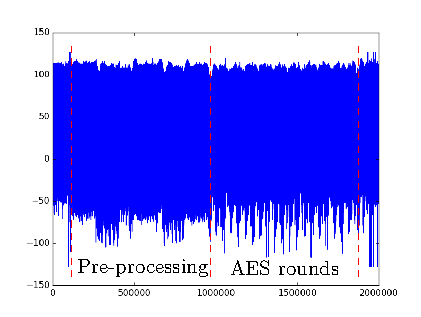
\includegraphics[scale=1]{figures/sample_traces_2M_label.pdf}
  \caption{Power consumption trace of the AES encryption.}
  \label{fig:sample_trace}
\end{figure}

No resynchronization step has been performed on these traces. Nonetheless, visual inspection indicates that no significant desynchronization occurs. To illustrate this, Figure~\ref{fig:3_traces} displays a temporal zoom on three different traces.

\begin{figure}[h]
	\centering 
	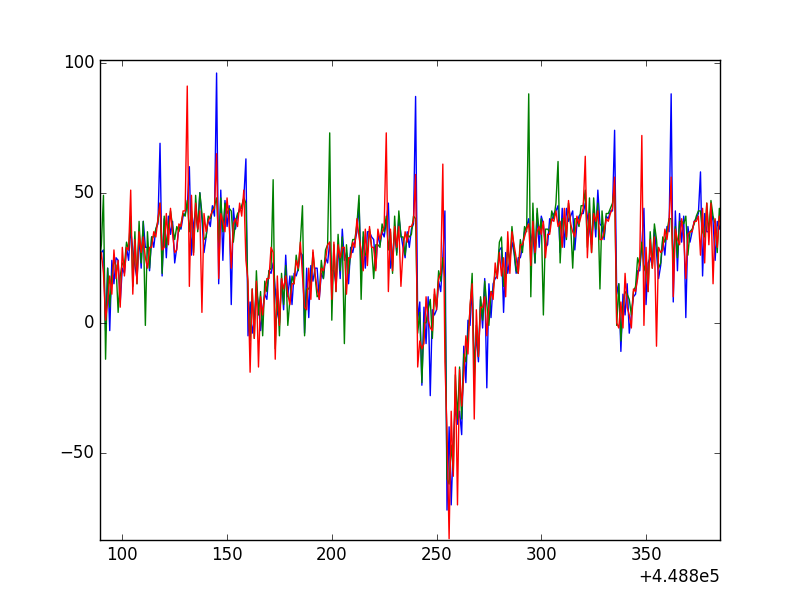
\includegraphics[scale=0.35]{figures/3_traces.png}
	\caption{Three traces on a short temporal window.}
	\label{fig:3_traces}
\end{figure}


A first acquisition campaign of $50.000$ traces of the rolled version (\emph{ie.}, the default version) is used to perform the caracterisation step as well as the first-order resilience assessment.
For the second and third order assessments, we used a second campaign of $100.000$ traces of the unrolled version. The following table summarizes the results.
The analyses are further detailed in the rest of this document.

\begin{figure}[h!]
\centering
\begin{tabular}{|c|c|c|c|c|c|c|}
  \hline
   & \multicolumn{3}{c|}{Known permutation}&\multicolumn{3}{c|}{Unknown permutation}\\
  \hline
  Known    & $\rmult, \rout$ & $\rmult $ &  None & $\rmult,\rout$ & $\rmult $  &  None \\
  \hline
  Order 1& $\approx 1.000$ & $ > 50.000$ & $> 50.000$& $\approx 20.000$ & $ > 50.000$ & > $50.000$\\
  \hline
  Order 2& N/A & $ > 8.000$ & $> 100.000$& N/A & $ > 100.000$ & > $100.000$\\
  \hline
  Order 3& N/A & N/A & $> 100.000$& N/A & N/A & > $100.000$\\
  \hline
\end{tabular}
\caption{Number of traces needed for a successful first-order, second-order, and thirs-order attack, depending on the masks known to the attacker.}
\end{figure}




\section{Secured AES: Affine masking}
\label{sec:secured_aes}
The version of the AES is an affine implementation according to the paper \emph{Affine masking against high-order side channel analysis}~\cite{FMPR10a}. 
Each byte state of the AES state, denoted $\statea[i]$ for the $i$-th byte, is manipulated under the form $\rmult \times \statea[i] \oplus \stateb[i]$: $\rmult$ is a non zero random byte, $\stateb[i]$ is initialized with 16-random bytes denoted $\maes[0]\dots \maes[15]$, and $\times$ denotes the multiplication over the AES finite field~\cite{FIPS197}. 
For each round, the AES operations are applied to both $\statea$ and $\stateb$.

Similarly, the key schedule operation is also protected by manipulating each byte of the key state, denoted  $\stateK[i]$, under an affine form $\rmult' \times \stateK[i] \oplus \keym[i]$ where $\keym$ is initialize with 16-random bytes denoted $ \mkey[0] \dots \mkey[15]$ independent from the aes random bytes $\maes[0]\dots \maes[15]$. As the key schedule is performed independently from encryption and decryption operations, before using each masked key byte,
it has to be changed into $\rmult \times \stateK[i] \oplus \keym[i]$ (same multiplicative byte $\rmult$) to have a consistent computation. 

To sum up, the AES encryption/decryption and the key schedule each use 19 random bytes as input:
\begin{itemize}
\item 16 bytes for Boolean masking $\maes[0]\dots \maes[15]$/$\mkey[0]\dots \mkey[15]$ that initialized the masking state $\stateb$/$\stateK$;
\item 1 multiplicative byte $\rmult$/$\rmult'$;
\item 2 bytes $\rin $, $\rout$ / $\rin'$, $\rout'$ (two boolean masking bytes used for SubByte operation). 
\end{itemize}
  
To make this report more readable, we provide the correspondance Table ~\ref{tab:notations} between the notations  in this report (``Here'') and in the ``assembly code''.  

\begin{center}

\begin{tabular}{lll}
	  Assembly code & Here & size \\ \hline
%	 raw key  & \texttt{t} & $\key$ & 16\\
\texttt{key\_rin[0]} 		& $\rin'$ 		& 1\\
 \texttt{key\_rout[0]} 		& $\rout '$ 	&1\\
\texttt{key\_rmult[0]} 		& $\rmult ' $	&1\\
 \texttt{key\_maskedState[i]} 	& $ \rmult \times \stateK[i] \oplus \keym[i] $ & 1\\
 \texttt{key\_masksState[i]} 	& $ \keym[i]$ & 1\\
\texttt{key\_gtab} 			& $\gtab$  	&$ 16 \times 16$ \\
\texttt{key\_permIndicesMC} &$\perMC$ & 4\\
\hline
 \texttt{aes\_state[i]} & $\rmult \times \statea[i] \oplus \stateb[i] $ & 1\\
 \texttt{aes\_state2[i]} & $\stateb[i]$  & 1\\
\texttt{aes\_rin[0]} & $\rin$ &1\\
\texttt{aes\_rout[0]} & $\rout$ &1\\
\texttt{aes\_rmult[0]} & $\rmult$ &1\\
 \texttt{aes\_gtab} &  $\gtab$  &$ 16 \times 16$\\
 \texttt{aes\_permIndices} & $\permIndices$& 16\\
\texttt{aes\_permIndicesBis} & $\permIndicesbis$ & 16\\
\texttt{aes\_permIndicesMC} & $\perMC$  & 4 \\
 \texttt{aes\_permIndicesBisMC} & $\perMCbis$  &4 \\
 \texttt{aes\_sboxMasked} & $\sboxm$ & $16 \times 16$ \\
\hline
\end{tabular}
\captionof{table}{Notations correspondance between this report and the assembly code. Sizes are in number of bytes.}
\label{tab:notations}
\end{center}


\noindent We can distinguish three main steps: 
\begin{itemize}

	\item[1] Pre-processing: before the AES rounds, the following operations in this order are performed : loading of inputs, computation of the table $\gtab$ (multiplication by $\rmult$), computation of the affine sbox denoted $\sboxm$, key schedule with affine masking.  
	
	\item[2] AES rounds: 10 AES rounds with affine masking of the state and subkeys.
	
	\item[3] Post-processing: after AES rounds, the state $\statea$ is unmasked by removing the Boolean mask $\stateb$ and by removing the multiplicative factor $\rmult$ (multiplying by $\rmult^{-1}$).
\end{itemize}

\noindent \underline{Shuffling:} Many sub-operations on the AES state are performed in a random order: each byte is processed in a random order with pre-computed permutation based on the input random values.
For AES rounds:
$\perMC$ is used to shuffle MixColumns of $\statea$ and $\perMCbis$ to shuffle MixColumns of $\stateb$. These permutations are computed from the initial value $\stateb[0]$.  
The permutation $\permIndices$ is used to shuffle SubBytes and ShiftRows of $\statea $ and the permutation $\permIndicesbis$ is used to shuffle SubBytes and ShiftRows of $\stateb$. These permutations are computed from $\maes[0], \maes[1], \maes[2], \maes[3]$.
%the initial value of $\stateb[0],$ $ \stateb[1], \stateb[2]$ and $\stateb[3]$.

For key schedule: the four permutations are similar. 
The permutation $\perMC$ is used to shuffle MixColumns of the masked key state and $\perMCbis$ to shuffle MixColumns of $\keym$. These permutations are computed from $\mkey[0]$. 
%the initial $\keym[0]$ value.  
The permutation $\permIndices$ is used to shuffle SubBytes and ShiftRows of the masked key state and $\permIndicesbis$ is used to shuffle SubBytes and ShiftRows of the key mask state $\keym$. These permutations are computed from $\mkey[0], \mkey[1], \mkey[2], \mkey[3]$.
%the initial values of $\keym[0], \keym[1], \keym[2]$ and $\keym[3]$.







\section{Characterization phase}
In this section, we perform several Signal-to-Noise Ratio (SNR) computations in order to identify univariate leakage samples related to the manipulation of different sensitive values.

\subsection{Key bytes}
We perform a SNR targeting each key byte.
We superpose the leakage and SNR curves for the first key byte in Figure~\ref{fig:SNR_K0} to locate where the SNR peaks are located during AES computation.
For each key byte, the results evidence one leakage point, which highlights the key manipulation during its masking (\texttt{Load\_masterKey} function).

\begin{figure}[H]
	\centering 
	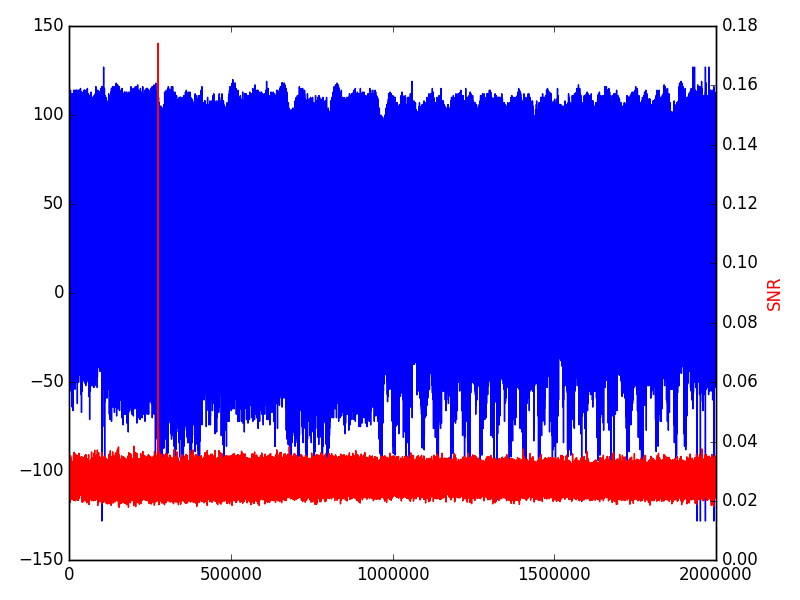
\includegraphics[scale=0.35]{figures/2Mpts/SNRK0_10ktraces.png}
	\caption{SNR targeting key byte 0 (in red), superposed to one leakage trace. SNR computed using $10.000$ traces.}
	\label{fig:SNR_K0}
\end{figure}

\subsection{Plaintext bytes}
Similarly, we perform a SNR targeting each plaintext byte as shown in Figure~\ref{fig:SNR_P0}. 
The results evidence three leakage points. The first leakage is explained by the loading of the plaintext in the target.
The second leakage is explained by the loading of the plaintext in the context (\texttt{Load\_data} function).
The third leakage is explained by the masking of the plaintext (\texttt{Map\_in\_G} function).

\begin{figure}[H]
	\centering 
	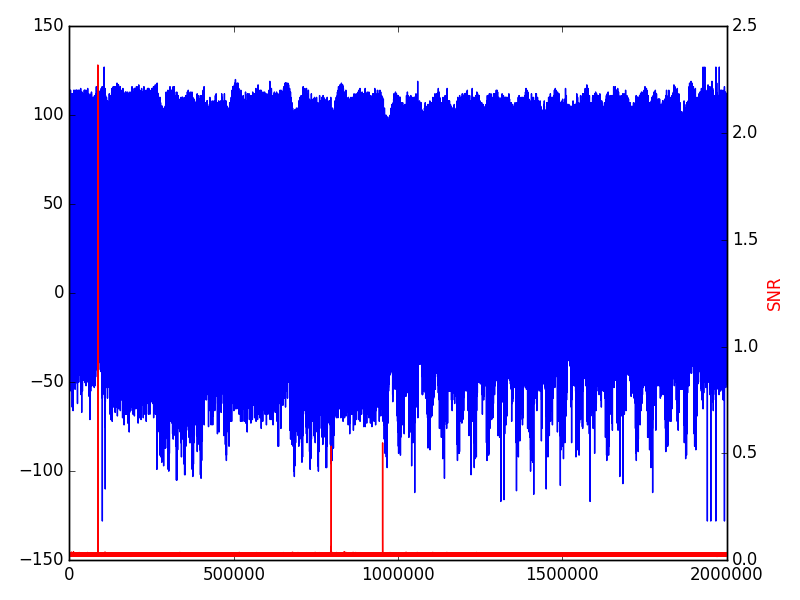
\includegraphics[scale=0.35]{figures/2Mpts/SNRP0_10ktraces.png}
	\caption{SNR targeting plaintext byte 0 (in red), superposed to one leakage trace. SNR computed using $10.000$ traces.}
	\label{fig:SNR_P0}
\end{figure}

\subsection{Ciphertext bytes}
Similarly, we perform a SNR targeting ciphertext bytes as shown in Figure~\ref{fig:SNR_C0}.
Leakages appear during the unmasking operation (\texttt{Multiplicative\_unmasking} function) and the serial writing of the bytes: when the ciphertext is loaded in the output variable.  %Note that the leakages occuring due to the serial writing do not appear for bytes 7 and plus, because of the limited trace size.

\begin{figure}[H]
	\centering 
	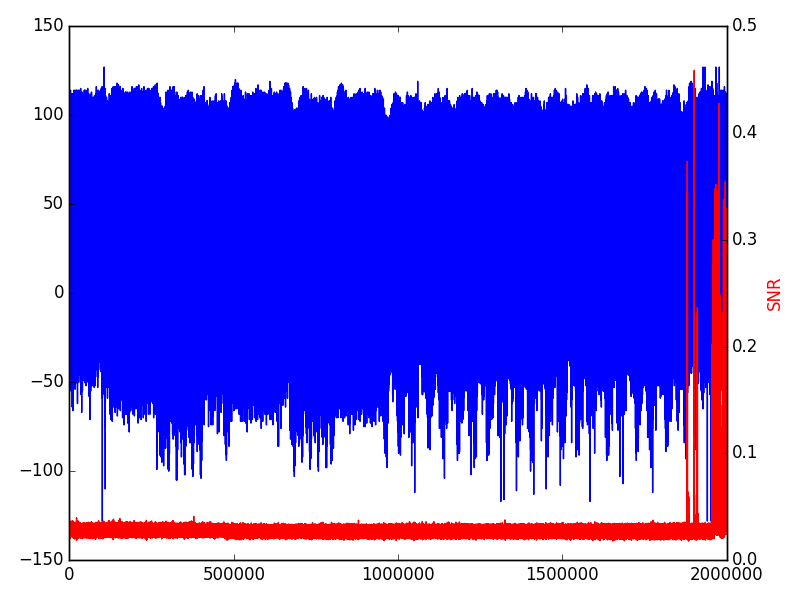
\includegraphics[scale=0.35]{figures/2Mpts/SNRC0_10ktraces.png}
	\caption{SNR targeting ciphertext byte 0 (in red), superposed to one leakage trace. SNR computed using $10.000$ traces.}
	\label{fig:SNR_C0}
\end{figure}

\subsection{Mask bytes}
Similarly, we perform a SNR targeting each mask byte. We detail the results hereafter, depending on the usages of each mask in the implementation.

\subsubsection{State masks}
Bytes $\maes[0]$ to $\maes[15]$, $\rin$, $\rout$ and $\rmult$ are used for the masking of the state of the encryption. We characterize hereafter their leakages.
 
Figure~\ref{fig:SNR_M0} and Figure~\ref{fig:SNR_M1} illustrate the results when targeting bytes $\maes[0]$ and $\maes[1]$. 
These bytes are used for computing both the shuffling permutation used in the substitution layer of the AES, and the permutations used in the linear layer. 
They are also used as linear masks.
Leakages appear during the loading of the bytes (\texttt{Load\_random} function).
Then, leakages appear during the computation of the shuffling permutation of the substitution layer, \texttt{Compute\_permIndices\_Tables}, and the computation of the permutations in the linear layer (\texttt{Compute\_permIndices\_Tables\_MC} functions).
Another leakage peak appears when the masks are loaded just before the encryption (\texttt{Load\_data} function), and a smaller peak appears when the state is masked (\texttt{Xor\_states} function).
Finally, we observe nine peaks corresponding to the 9 \texttt{MixColumns} operations.

\begin{figure}[H]
	\centering 
	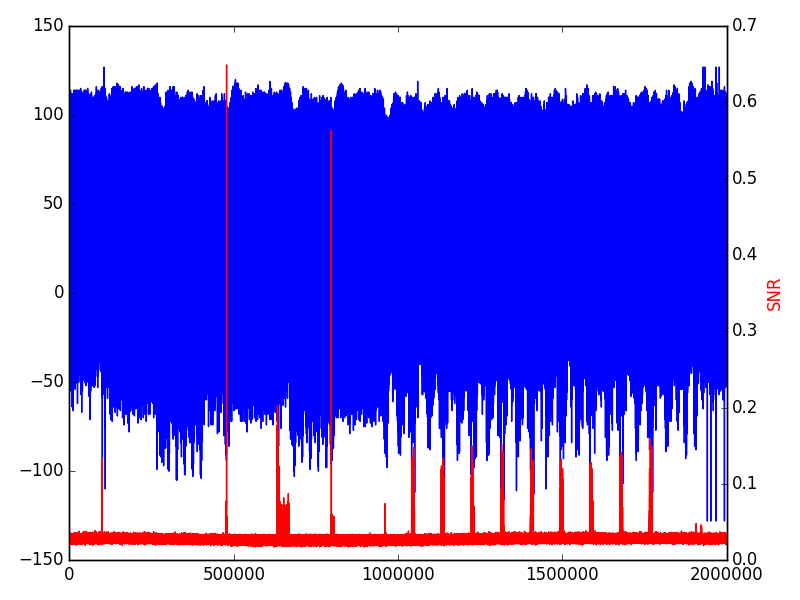
\includegraphics[scale=0.35]{figures/2Mpts/SNR_M0_10ktraces.png}
	\caption{SNR targeting mask byte $\maes[0]$ (in red), superposed to one leakage trace. SNR computed using $10.000$ traces.}
	\label{fig:SNR_M0}
	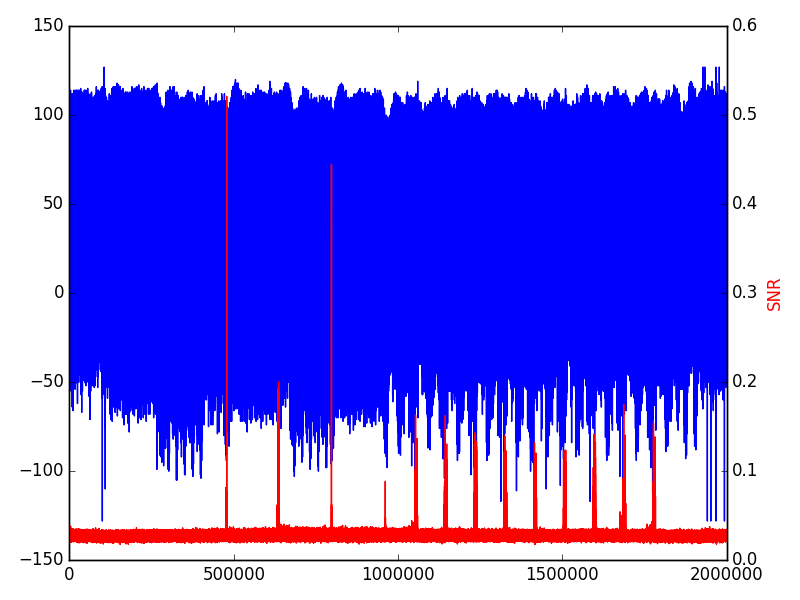
\includegraphics[scale=0.35]{figures/2Mpts/SNR_M1_10ktraces.png}
	\caption{SNR targeting mask byte $\maes[1]$ (in red), superposed to one leakage trace. SNR computed using $10.000$ traces.}
	\label{fig:SNR_M1}
\end{figure}

Figures~\ref{fig:SNR_M2} and~\ref{fig:SNR_M3} illustrate the results when targeting bytes $\maes[2]$ and $\maes[3]$. 
These bytes are used for computing the shuffling permutation used in the substitution layer, and as linear masks.
The leakages are similar to those of bytes $\maes[0]$ and $\maes[1]$, except that no leakage is observed during the \texttt{MixColumns} operations, nor during the computation of the permutations used in the linear layer.

\begin{figure}[H]
	\centering 
	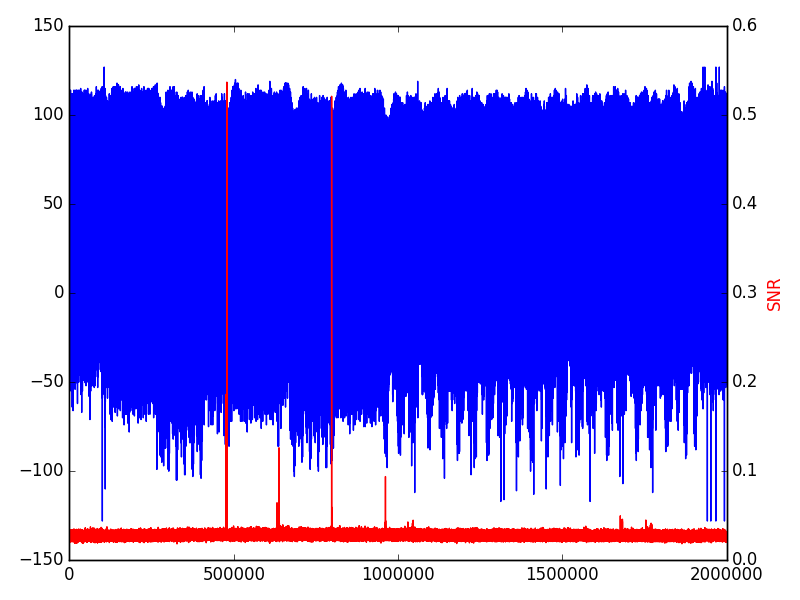
\includegraphics[scale=0.35]{figures/2Mpts/SNR_M2_10ktraces.png}
	\caption{SNR targeting mask byte $\maes[2]$ (in red), superposed to one leakage trace. SNR computed using $10.000$ traces.}
	\label{fig:SNR_M2}
	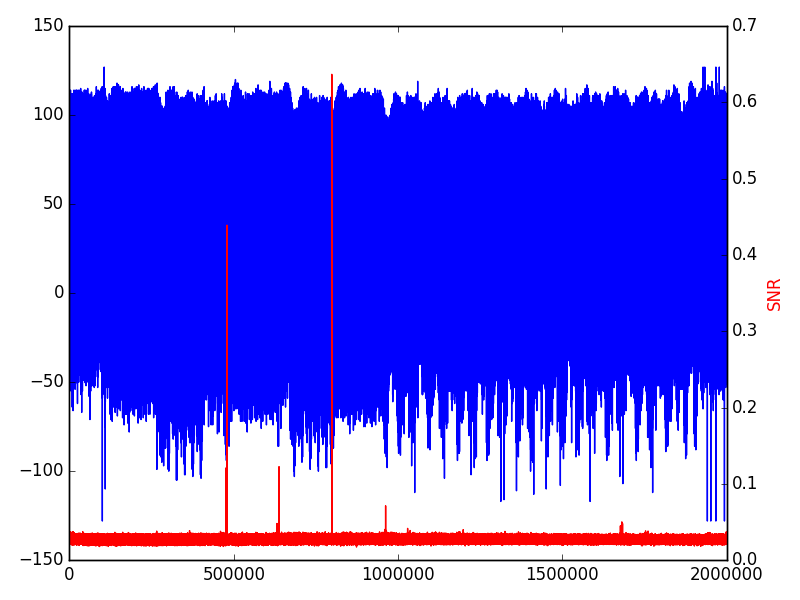
\includegraphics[scale=0.35]{figures/2Mpts/SNR_M3_10ktraces.png}
	\caption{SNR targeting mask byte $\maes[3]$ (in red), superposed to one leakage trace. SNR computed using $10.000$ traces.}
	\label{fig:SNR_M3}
\end{figure}

Figures~\ref{fig:SNR_M4} and \ref{fig:SNR_M15} illustrate the results when targeting bytes $\maes[4]$ and $\maes[15]$. These bytes are used as linear masks. Similar results are obtained for bytes $\maes[5]$ to $\maes[14]$.
The leakages are similar to the one obtained for previous bytes, but are now only observed for the loadings and masking of the state.
\begin{figure}[H]
	\centering 
	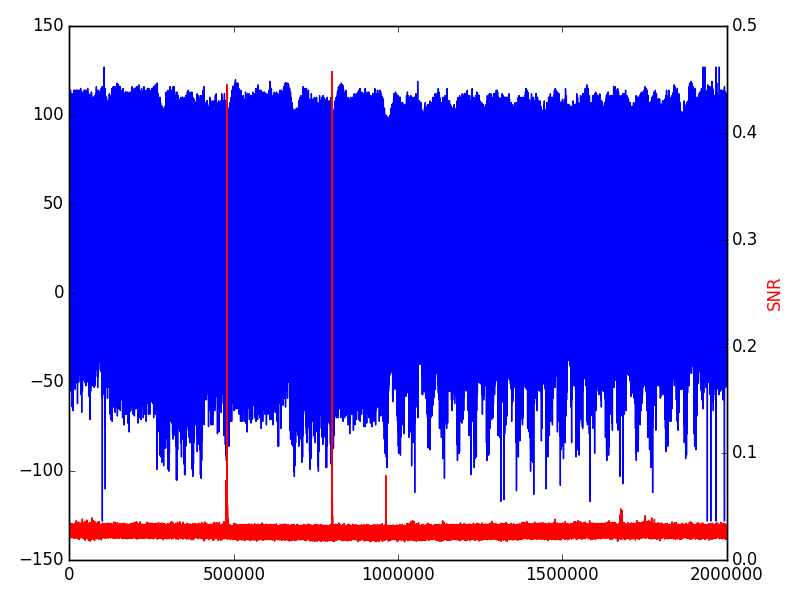
\includegraphics[scale=0.35]{figures/2Mpts/SNR_M4_10ktraces.png}
	\caption{SNR targeting mask byte $\maes[4]$ (in red), superposed to one leakage trace. SNR computed using $10.000$ traces.}
	\label{fig:SNR_M4}
	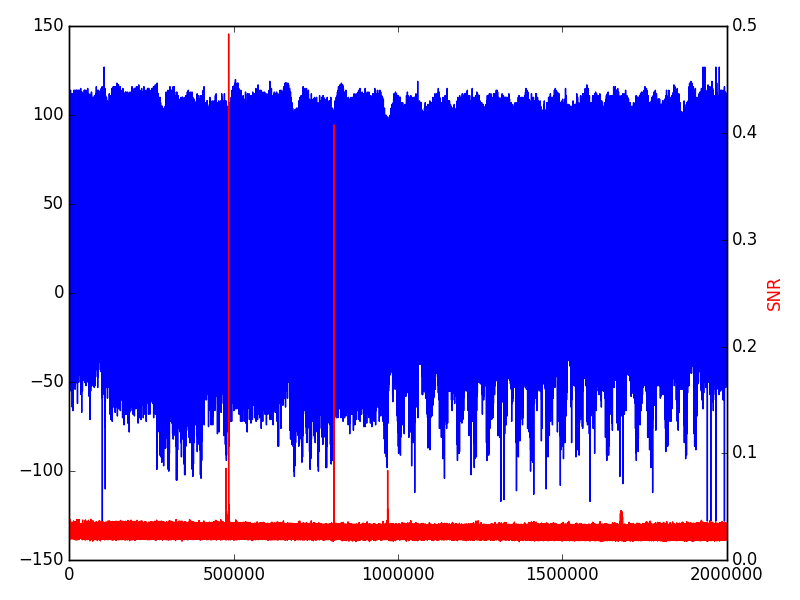
\includegraphics[scale=0.35]{figures/2Mpts/SNR_M15_10ktraces.png}
	\caption{SNR targeting mask byte $\maes[15]$ (in red), superposed to one leakage trace. SNR computed using $10.000$ traces.}
	\label{fig:SNR_M15}
\end{figure}

Figure~\ref{fig:SNR_rin} illustrates the results when targeting $\rin$. This byte is used as the input mask of the substition layer. 
Leakage first appears during the loading of the randoms (\texttt{Load\_data}).
Strong leakage can then be observed during the recomputation of the substitution table (\texttt{Compute\_Affine\_sboxMasked} function).
Finally 10 peaks appear during the substitution steps of each round of the AES.
\begin{figure}[H]
	\centering 
	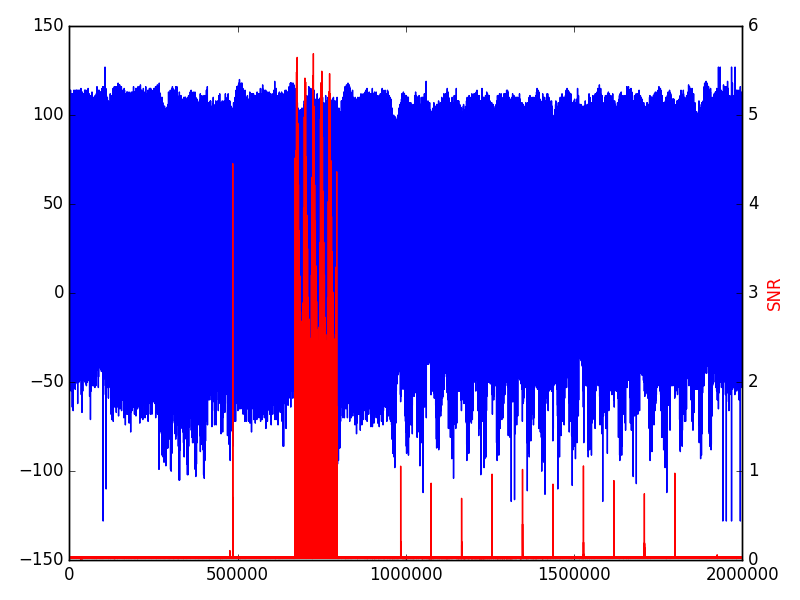
\includegraphics[scale=0.35]{figures/2Mpts/SNR_M16_10ktraces.png}
	\caption{SNR targeting mask byte $\rin $ (in red), superposed to one leakage trace. SNR computed using $10.000$ traces.}
	\label{fig:SNR_rin}
\end{figure}

Figure~\ref{fig:SNR_beta} illustrates the results when targeting $\rout$. This byte is used as the output mask of the subtitution layer. 
Leakages appear at similar time samples as for $\rin$.
\begin{figure}[H]
	\centering 
	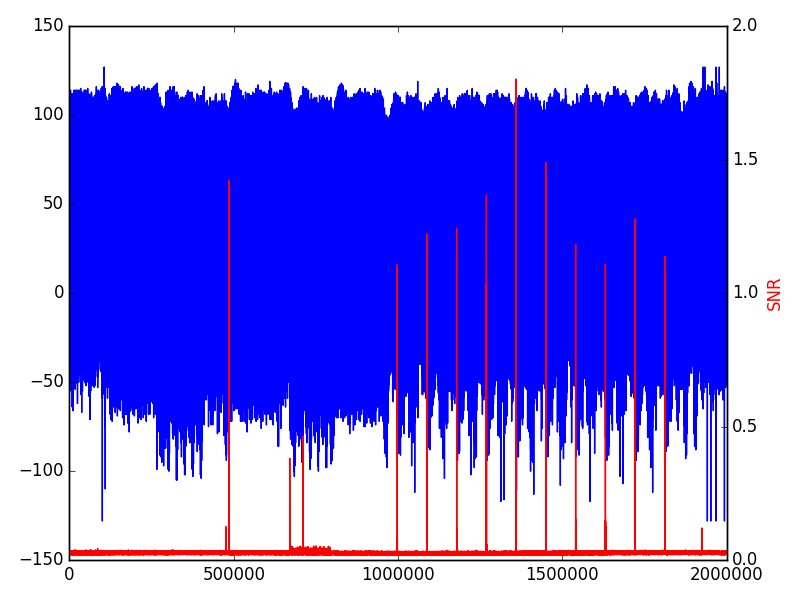
\includegraphics[scale=0.35]{figures/2Mpts/SNR_M17_10ktraces.png}
	\caption{SNR targeting mask byte $\rout$ (in red), superposed to one leakage trace. SNR computed using $10.000$ traces.}
	\label{fig:SNR_beta}
\end{figure}

Figure~\ref{fig:SNR_alpha} illustrates the results when targeting $\rmult$. This byte is used as the multiplicative mask of the substitution layer.
Leakage once again appear when the randoms are loaded (\texttt{Load\_data} function).
Leakage also appear during the computation of the multiplicative table (\texttt{Compute\_GTab} function), and during the computation of the substitution box (\texttt{Compute\_Affine\_sboxMasked} function).
\begin{figure}[H]
	\centering 
	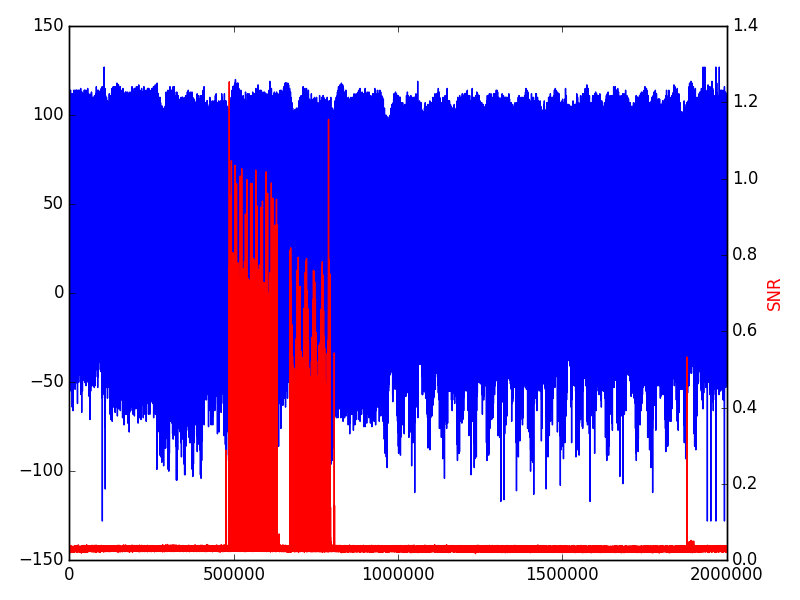
\includegraphics[scale=0.35]{figures/2Mpts/SNR_M18_10ktraces.png}
	\caption{SNR targeting mask byte $\rmult$ (in red), superposed to one leakage trace. SNR computed using $10.000$ traces.}
	\label{fig:SNR_alpha}
\end{figure}

\subsubsection{Key masks}
Bytes $\mkey[0]$ to $\mkey[15]$, $\rin'$, $\rout'$ and $\rmult'$ are used for the masking of the key. We characterize hereafter their leakages.
Figure~\ref{fig:SNR_M19} illustrates the results when targeting byte $\mkey[0]$. 
These bytes are used for computing the shuffling permutation used in the key expansion.
They are also used as linear masks.

Observed peaks correspond to the loading of the random in the target, loading of the masks (\texttt{Load\_random\_key} function), masking of the key (\texttt{Load\_masterKey}),
and the key expansion (\texttt{KeyExpansion\_masked} function), due to the involvment of the mask byte in the computation of the shuffling permutation\\ (\texttt{Compute\_permIndices\_Tables\_MC} function).

\begin{figure}[H]
	\centering 
	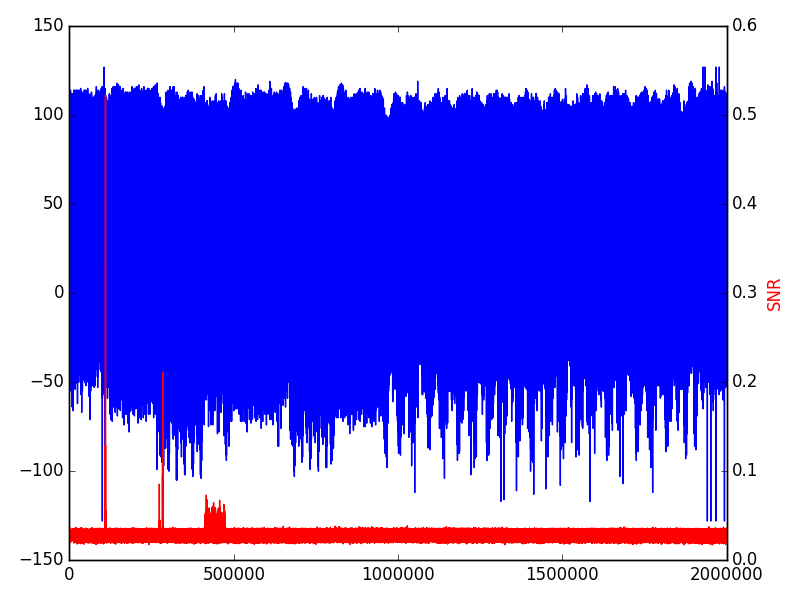
\includegraphics[scale=0.35]{figures/2Mpts/SNR_M19_10ktraces.png}
	\caption{SNR targeting mask byte $\mkey[0]$ (in red), superposed to one leakage trace. SNR computed using $10.000$ traces.}
	\label{fig:SNR_M19}
\end{figure}

Figures~\ref{fig:SNR_M20} and~\ref{fig:SNR_M21} illustrate the results when targeting bytes $\mkey[1]$ and $\mkey[2]$.  Similar results are observed when targeting bytes $\mkey[3]$ to $\mkey[15]$.
These bytes are not used for the computation of the shuffling permutation. However, they  serve as linear masks during the key expansion, and, as such, a small peak appears at the beginning of the \texttt{KeyExpansion\_masked} function.
The other peaks are similar to the ones appearing for byte $\mkey[0]$.

\begin{figure}[H]
	\centering 
	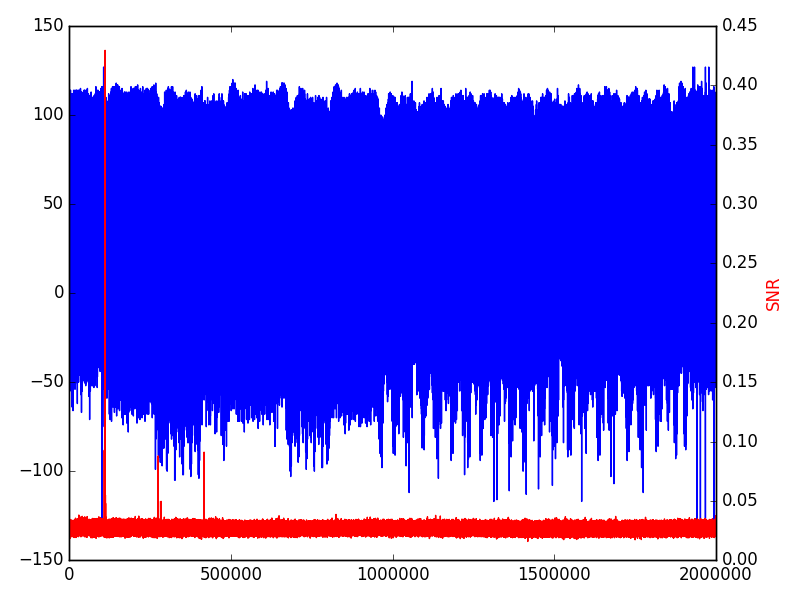
\includegraphics[scale=0.35]{figures/2Mpts/SNR_M20_10ktraces.png}
	\caption{SNR targeting mask byte $\mkey[1]$ (in red), superposed to one leakage trace. SNR computed using $10.000$ traces.}
	\label{fig:SNR_M20}
	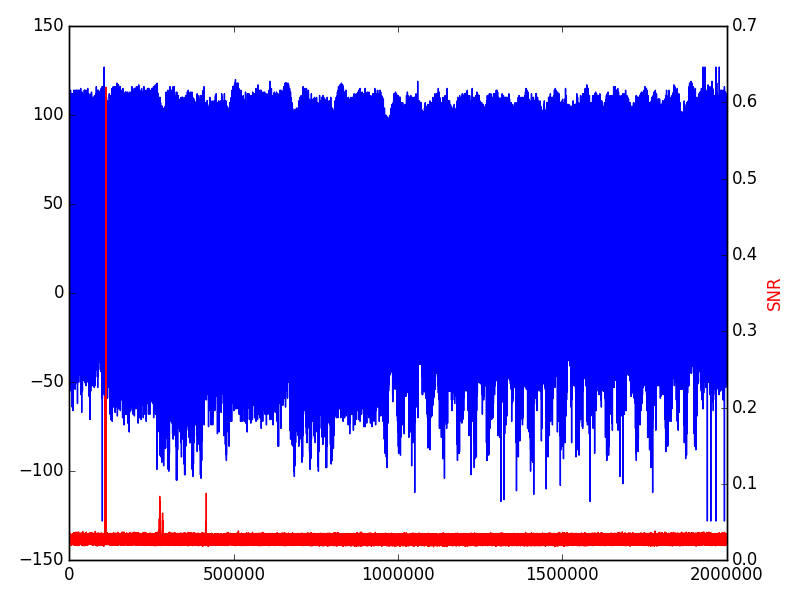
\includegraphics[scale=0.35]{figures/2Mpts/SNR_M21_10ktraces.png}
	\caption{SNR targeting mask byte $\mkey[2]$ (in red), superposed to one leakage trace. SNR computed using $10.000$ traces.}
	\label{fig:SNR_M21}
\end{figure}


Figure~\ref{fig:SNR_rin2} illustrates the results when targeting $\rin'$. This byte is used as the input mask of the substition layer.
Leakages appear at the same time samples as for bytes $\mkey[1]$ to $\mkey[15]$, and also during the recomputation of the Sbox and the key expansion.
\begin{figure}[H]
	\centering 
	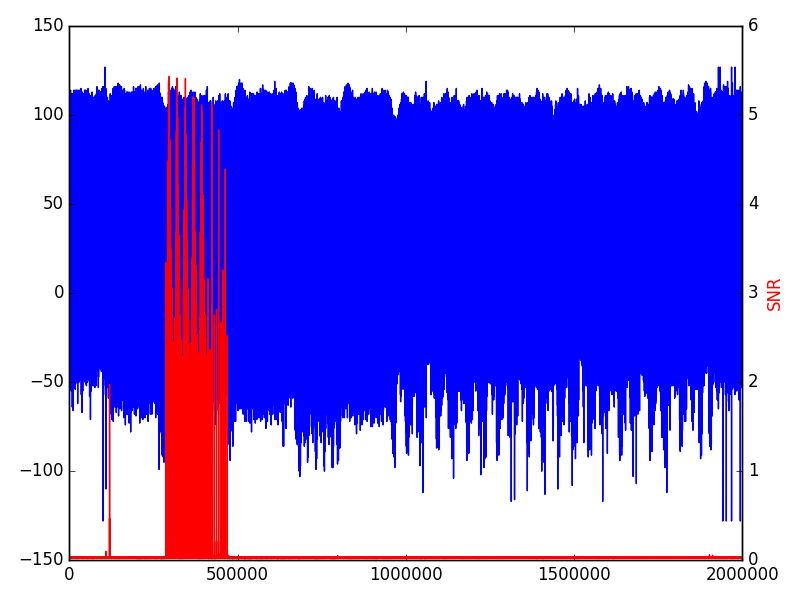
\includegraphics[scale=0.35]{figures/2Mpts/SNR_M35_10ktraces.png}
	\caption{SNR targeting mask byte $\rin'$ (in red), superposed to one leakage trace. SNR computed using $10.000$ traces.}
	\label{fig:SNR_rin2}
\end{figure}

Figure~\ref{fig:SNR_beta2} illustrates the results when targeting $\rout'$. This byte is used as the output mask of the subtitution layer. 
Leakages appear at the same time samples as for bytes $\mkey[1]$ to $\mkey[15]$, and also during the recomputation of the Sbox and the key expansion.
\begin{figure}[H]
	\centering 
	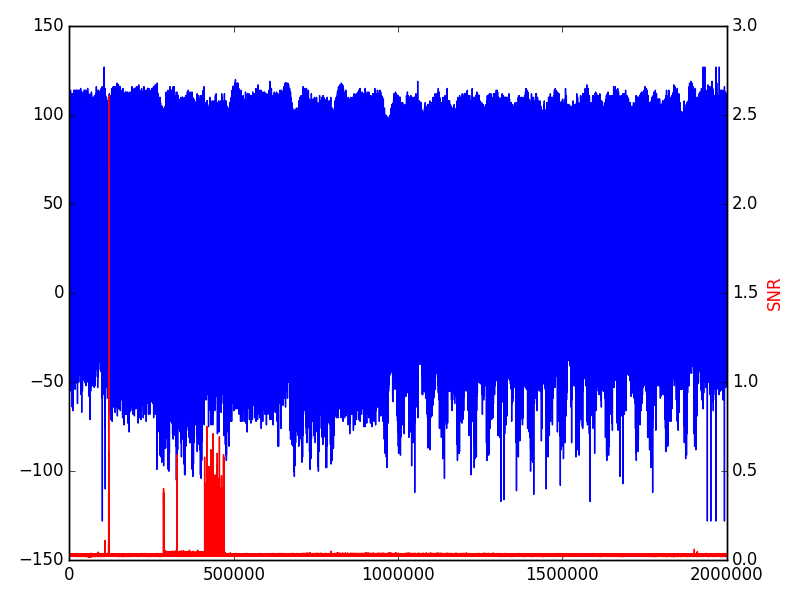
\includegraphics[scale=0.35]{figures/2Mpts/SNR_M36_10ktraces.png}
	\caption{SNR targeting mask byte $\rout'$ (in red), superposed to one leakage trace. SNR computed using $10.000$ traces.}
	\label{fig:SNR_beta2}
\end{figure}

Figure~\ref{fig:SNR_alpha2} illustrates the results when targeting byte $\rmult'$. This byte is used as the multiplicative mask of the substitution layer.
Leakages appear at the same time samples as the previous bytes, and also during the computation of the multiplication table \texttt{Gtab}.
Finally, a peak appears just before the encryption, when the value is loaded.
\begin{figure}[H]
	\centering 
	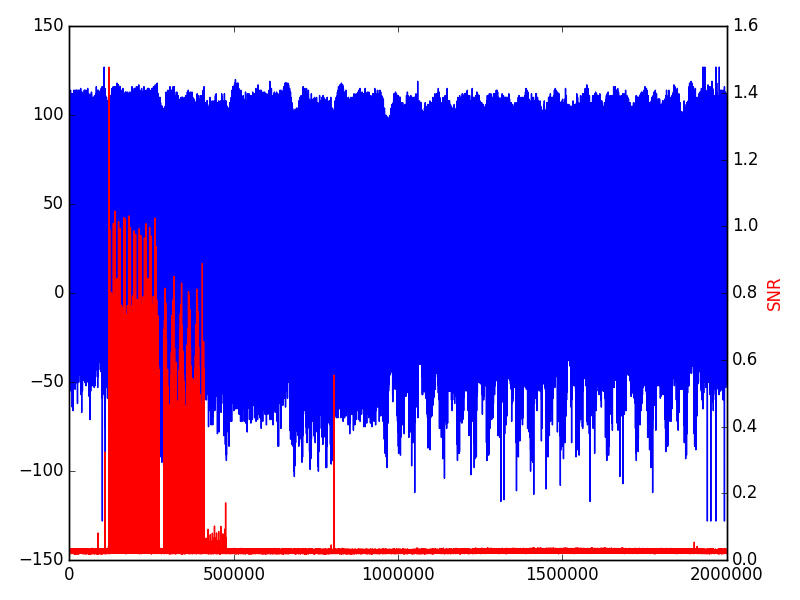
\includegraphics[scale=0.35]{figures/2Mpts/SNR_M37_10ktraces.png}
	\caption{SNR targeting mask byte $\rmult'$ (in red), superposed to one leakage trace. SNR computed using $10.000$ traces.}
	\label{fig:SNR_alpha2}
\end{figure}

\subsection{Sbox output bytes}
\subsubsection{Raw bytes}
Figure~\ref{fig:SNR_S0} illustrates the results when targeting a Sbox output byte without taking into account the output mask (ie. for each byte $i$, the value $S[\plain[i]\oplus \key[i]]$ is targeted) and there is no observable leakage.
\begin{figure}[H]
	\centering 
	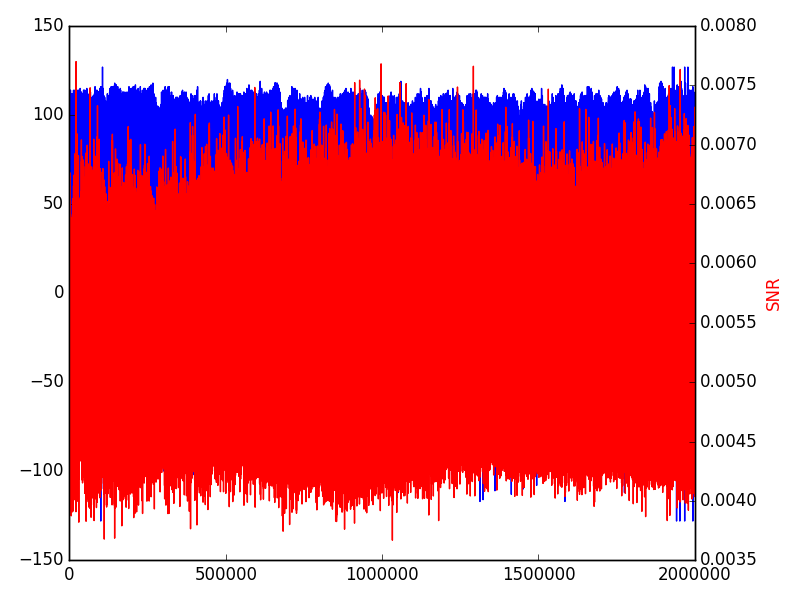
\includegraphics[scale=0.35]{figures/2Mpts/SNR_raw_S0_50ktraces.png}
	\caption{SNR targeting Sbox output byte 0 (in red), superposed to one leakage trace. SNR computed using $50.000$ traces.}
	\label{fig:SNR_S0}
\end{figure}

\subsubsection{Multiplied by mask} 
Figure~\ref{fig:SNR_aS0} illustrates the results when targeting a byte of the Sbox output, multiplied by the multiplicative mask, ie., for each byte $i$, the value $\rmult \times S[\plain[i]\oplus \key[i]]$ is targeted. No significant leakage is observed.
\begin{figure}[H]
	\centering 
	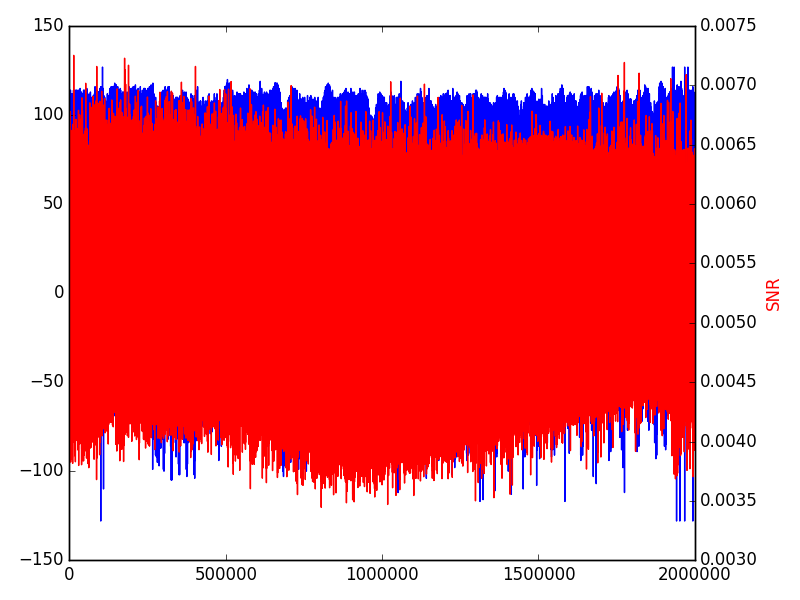
\includegraphics[scale=0.35]{figures/2Mpts/SNR_raw_aS0_50ktraces.png}
	\caption{SNR targeting the multiplicatively masked Sbox output byte 0 (in red), superposed to one leakage trace. SNR computed using $50.000$ traces.}
	\label{fig:SNR_aS0}
\end{figure}

\subsubsection{Affine masked}
Figure~\ref{fig:SNR_aS0+b} illustrates the results when targeting a byte of the Sbox output, affinely masked, ie., for each byte $i$, the value $\rmult \times S[P[i]\oplus K[i]] \oplus \rout$ is targeted. We remark that $50.000$ traces are not enough to highlight a leakage of this value.
This result is expected because of the shuffling countermeasure.
\begin{figure}[H]
	\centering 
	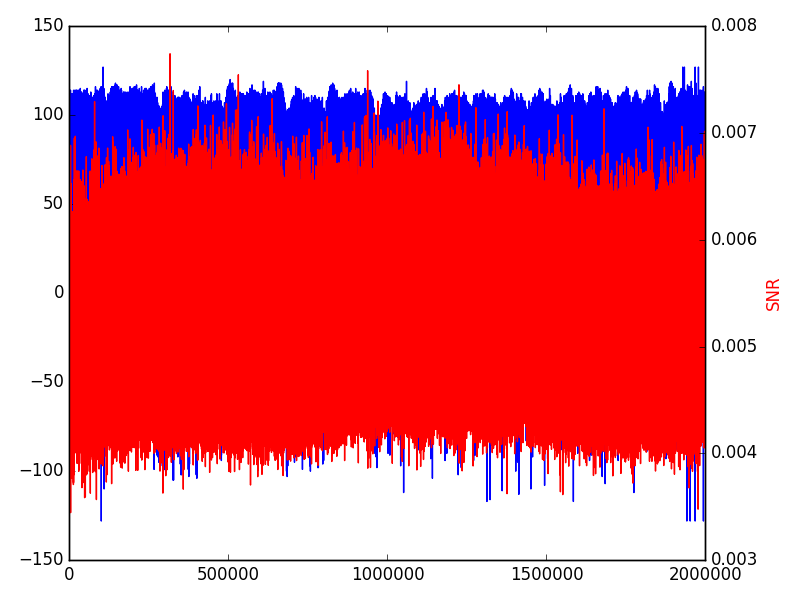
\includegraphics[scale=0.35]{figures/2Mpts/SNR_raw_aS+b0_50ktraces.png}
	\caption{SNR targeting the affinely masked Sbox output byte 0 (in red), superposed to one leakage trace. SNR computed using $50.000$ traces.}
	\label{fig:SNR_aS0+b}
\end{figure}


\subsection{Unshuffled output bytes}
\subsubsection{Raw bytes}
We use the knowledge of the mask bytes to inverse the shuffling $Sh$ performed during the substitution phase. For each index $i$, we target the value $S[\plain[Sh[i]]\oplus \key[Sh[i]]] $. No significant leakage can be observed. 
Figure~\ref{fig:SNR_unshuffledS0} illustrates the results.
\begin{figure}[H]
	\centering 
	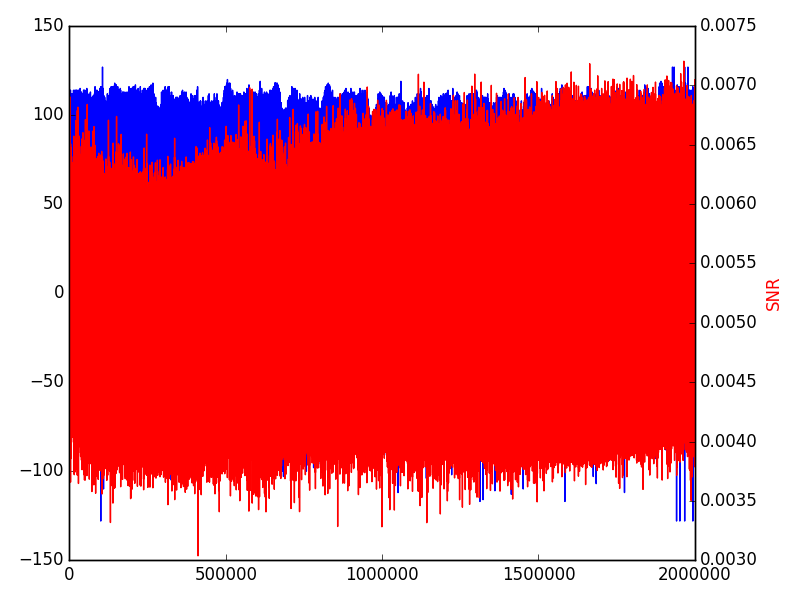
\includegraphics[scale=0.35]{figures/2Mpts/SNR_unshuffled_S0_50ktraces.png}
	\caption{SNR targeting the unshuffled Sbox output byte 0 (in red), superposed to one leakage trace. SNR computed using $50.000$ traces.}
	\label{fig:SNR_unshuffledS0}
\end{figure}

\subsubsection{Multiplicately masked}
We use the knowledge of the mask bytes to inverse the shuffling $Sh$ performed during the substitution phase. For each index $i$, we target the value $\rmult \times S[\plain[Sh(i)]\oplus \key[Sh(i)]]$. A small amount of leakage is present, at the time of the manipulation of $\rmult$. This is easily explained since the random variables $\rmult \times S[\plain[Sh(i)]\oplus \key[Sh(i)]]$ and $\rmult$ are not independent. 
Figure~\ref{fig:SNR_unshuffledaS0} illustrates the results.
\begin{figure}[H]
	\centering 
	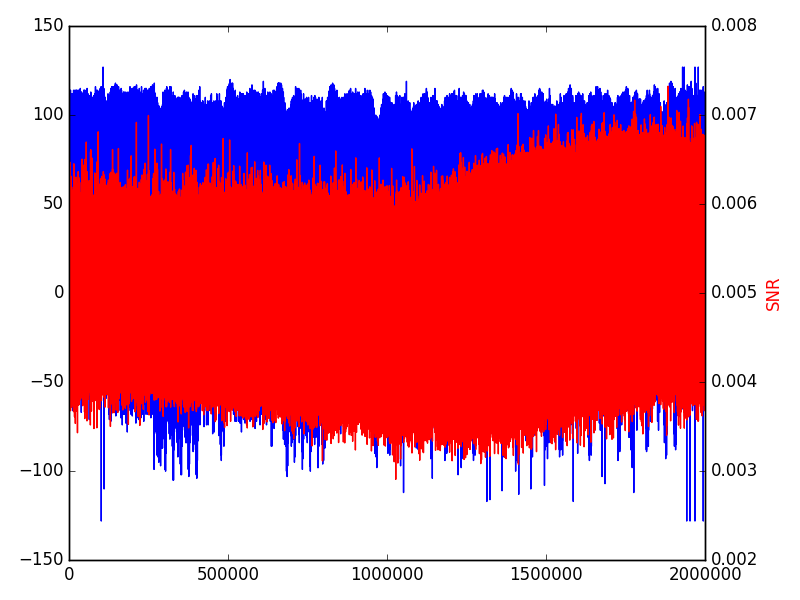
\includegraphics[scale=0.35]{figures/2Mpts/SNR_unshuffled_aS0_50ktraces.png}
	\caption{SNR targeting the unshuffled multiplicatively masked Sbox output byte 0 (in red), superposed to one leakage trace. SNR computed using $50.000$ traces.}
	\label{fig:SNR_unshuffledaS0}
\end{figure}

\subsubsection{Affinely masked}
We use the knowledge of the mask bytes to inverse the shuffling $Sh$ performed during the substitution phase. For each index $i$, we target the value $\rmult \times S[\plain[Sh(i)]\oplus \key[Sh(i)]] \oplus \rout$. A significant leakage is observed after the first substitution layer. %reprendre la notation pour le shuffle
Figure~\ref{fig:SNR_unshuffledaS0+b} illustrates the results.
\begin{figure}[H]
	\centering 
	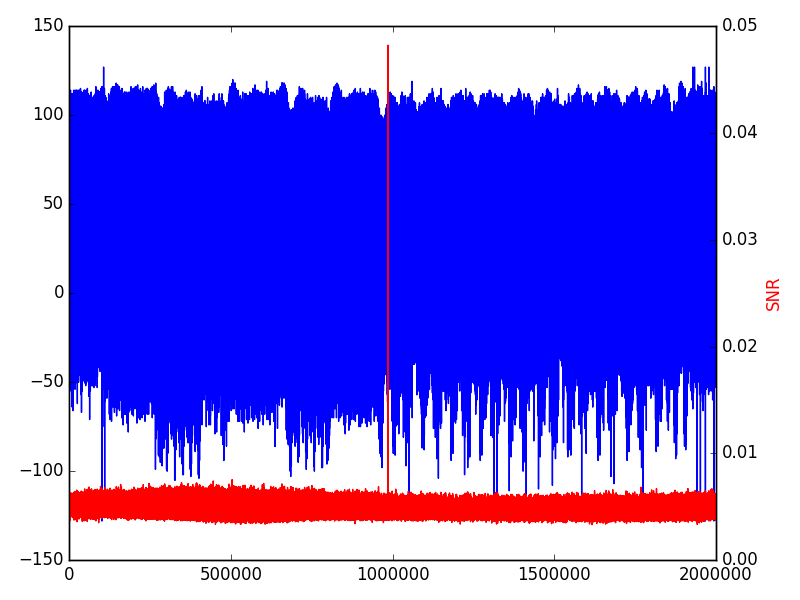
\includegraphics[scale=0.35]{figures/2Mpts/SNR_unshuffled_aS+b0_50ktraces.png}
	\caption{SNR targeting the unshuffled affinely masked Sbox output byte 0 (in red), superposed to one leakage trace. SNR computed using $50.000$ traces.}
	\label{fig:SNR_unshuffledaS0+b}
\end{figure}




\section{First-order correlation analysis}
In this section, we analyse the effectiveness of the implemented countermeasures against first-order side-channel analysis based on the linear correlation coefficient (Correlation Power Analysis CPA). For this study, we will target the Sbox output value. 

We separate this study in two parts. In the first part, we will characterize the effectiveness of a CPA against this implementation, by considering an attacker with priviledged knowledge. In the second part, we will evaluate the effectiveness of a CPA against this implementation without such knowledge.

\subsection{Priviledged knowledge}
We first study the setting where the attacker knows the random masks used to compute the permutation. 

In order to characterize the effectiveness of a CPA against this implemenation, we use the random masks to recompute the permutation $Sh(i)$ for each byte index $i$. We then perform an attack targeting the value 

\noindent $Z_{\hat{\key}}[i]=S[\plain[Sh(i)] \oplus \key[Sh(i)] \oplus \hat{\key}]$, where $\hat{\key}$ is an hypothesis on a value of one byte.
The attack is successful if the best hypothesis returned by the attack is $0$.

% Equivalently, $Z[i]=S[P[Sh(i)] \oplus K[Sh(i)] \oplus \hat{k} \oplus K[i]] and the best result is K[i]

\subsubsection{Affinely masked Sbox output}
We suppose the knowledge of both the multiplicative mask and the output mask. This knowledge allows for the prediction of the value $\rmult \times Z_{\hat{\key}}[i] \oplus \rout$ for any hypothesis $\key$. Depending on the index byte, the attack succeeds with around $1.000$ traces.
Figure~\ref{fig:CPA1O_trickedaZb1} illustrates the result of the attack targeting byte 0, using $1.000$ traces.

\begin{figure}[H]
	\centering 
	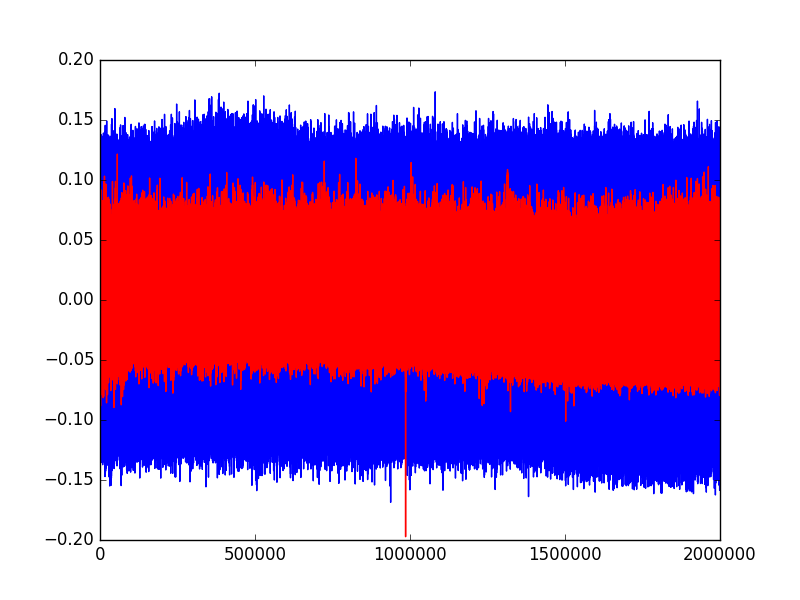
\includegraphics[scale=0.4]{figures/CPA1O_2Mpts_trickedaS+b0_1ktraces.png}
	\caption{Correlation coefficients obtained when targeting $\rmult \times Z_{\hat{\key}}[i] \oplus \rout$, for every value of $\hat{\key}$. Correct hypothesis is plotted  in red. }
	\label{fig:CPA1O_trickedaZb1}
\end{figure}

%attack_results_without_flaw_fixed_100k
\subsubsection{Multiplicatively masked Sbox output}
We suppose the knowledge of the multiplicative mask. This knowledge allows for the prediction of the value $\rmult \times Z_{\hat{\key}}[i]$ for any hypothesis $\hat{\key}$.
The attack is unsuccessful using $50.000$ traces.
Figure~\ref{fig:CPA1O_trickedaZ1} illustrates the result of the attack targeting byte 0, using $50.000$ traces.

\begin{figure}[H]
	\centering 
	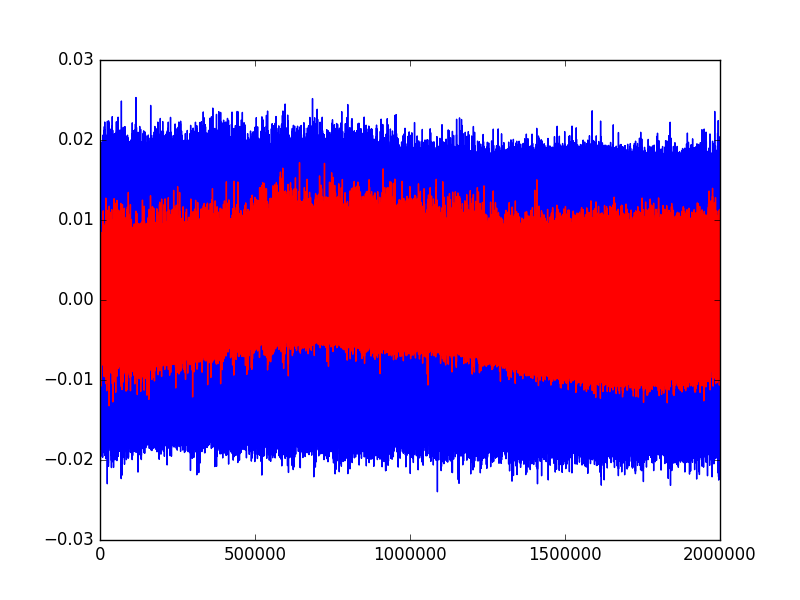
\includegraphics[scale=0.4]{figures/CPA1O_2Mpts_trickedaS0traces.png}
	\caption{Correlation coefficients obtained when targeting $\rmult \times Z_{\hat{\key}}[i]$, for every value of $\hat{\key}$. Correct hypothesis is plotted  in red. }
	\label{fig:CPA1O_trickedaZ1}
\end{figure}

%attack_results_without_flaw_fixed_100k
\subsubsection{Raw Sbox output}
We suppose no prior knowledge (except the permutation), and predict the value $Z_{\hat{\key}}[i]$ for any hypothesis $\hat{\key}$.
The attack is unsuccessful using $50.000$ traces.
Figure~\ref{fig:CPA1O_trickedZ1} illustrates the result of the attack targeting byte 0, using $50.000$ traces.

\begin{figure}[H]
	\centering 
	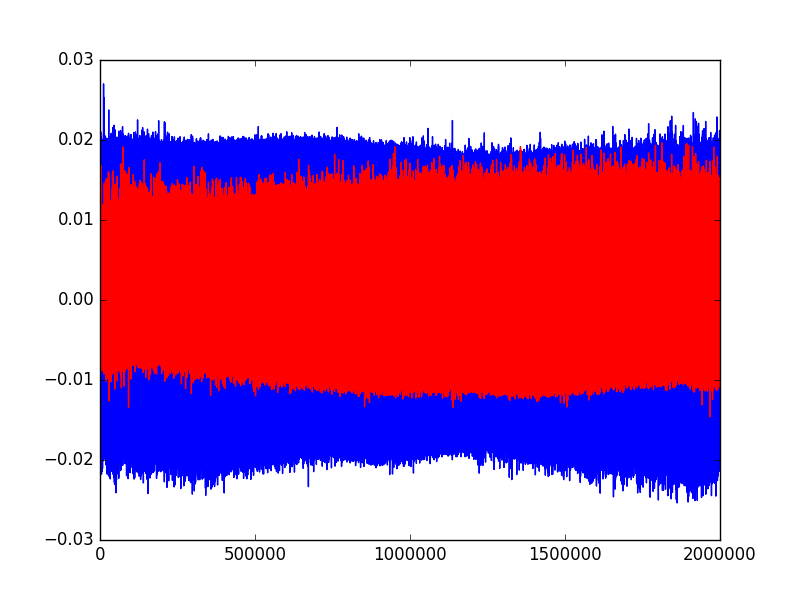
\includegraphics[scale=0.4]{figures/CPA1O_2Mpts_trickedS0traces.png}
	\caption{Correlation coefficients obtained when targeting $\rmult \times Z_{\hat{\key}}[i]$, for every value of $\hat{k}$. Correct hypothesis is plotted  in red. }
	\label{fig:CPA1O_trickedZ1}
\end{figure}

\subsection{Unknown permutation, processed traces}
We now study the setting where the attacker does not know the random masks used to compute the permutation.

We preprocess the traces in order to average the leakage over the different byte indices manipulation:
\begin{itemize}
	\item for each index $i$ in $[0,15]$, we define a small window $w_i$ of $\ell$ points around the SNR peak corresponding to the manipulation of $\rmult \times S[P[Sh(i)] \oplus K[Sh(i)]]\oplus \rout$ in the characterization phase. In our experiments, the size of the window was arbitrarily fixed to $\ell=11$.
	\item for each trace in our acquisition campaign, we compute the average window $m$ such that for each time sample $j$, $m[j]=\frac{1}{16}\sum_{i=0}^{15} w_i[j]$. We then consider $m$ as our reduced averaged trace of size $\ell$.
\end{itemize}

%/media/nas/projects/ASCAD_CW/ASCAD_ChipWhisperer/ARM/traces/averaged_attack_results_without_flaw_fixed_100k.h5
\subsubsection{Affinely masked Sbox output}
We suppose the knowledge of both the multiplicative mask and the output mask. This knowledge allows for the prediction of the value $\rmult \times S[\plain[i]\oplus \hat{\key}] \oplus \rout$ for any hypothesis $\hat{\key}$ on one byte of the secret key.
Depending on the byte index, the CPA is successful using around $20.000$ to $30.000$ traces.

Figure~\ref{fig:CPA1O_averaged_aZb1} illustrates the results using $50.000$ traces.
\begin{figure}[H]
	\centering 
	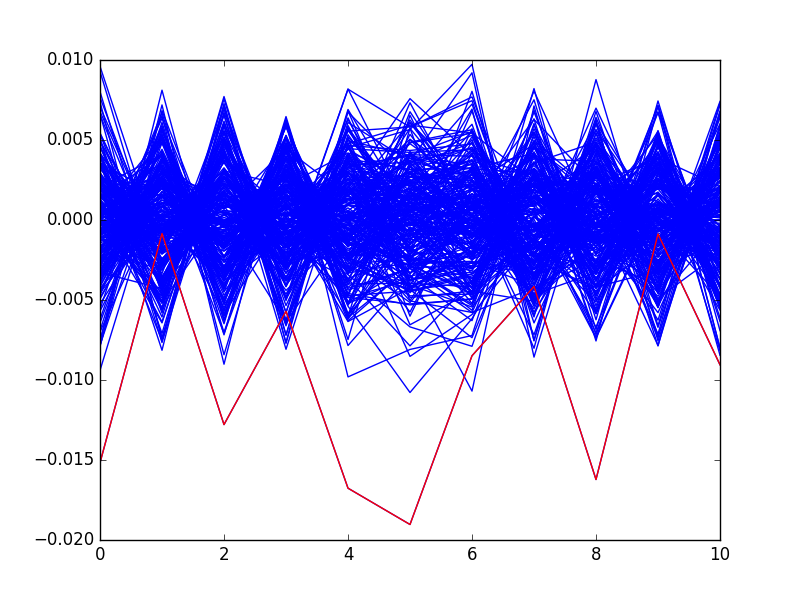
\includegraphics[scale=0.4]{figures/CPA1O_averaged_aZb1.png}
	\caption{Correlation coefficients obtained when targeting $\rmult \times S[\plain[i]\oplus \hat{\key}] \oplus \rout$, on averaged traces, for every value of $\hat{\key}$. Correct hypothesis is plotted  in red.}
	\label{fig:CPA1O_averaged_aZb1}
\end{figure}

\subsubsection{Multiplicatively masked Sbox output}
With $50.000$ traces, the attack does not succeed when targeting $\rmult \times S[\plain[i]\oplus \hat{\key}]$.
Figure~\ref{fig:CPA1O_averaged_aZ1} illustrates the results using $50.000$ traces.

Figure~\ref{fig:CPA1O_averaged_aZ1} illustrates the results using $50.000$ traces.
\begin{figure}[H]
	\centering 
	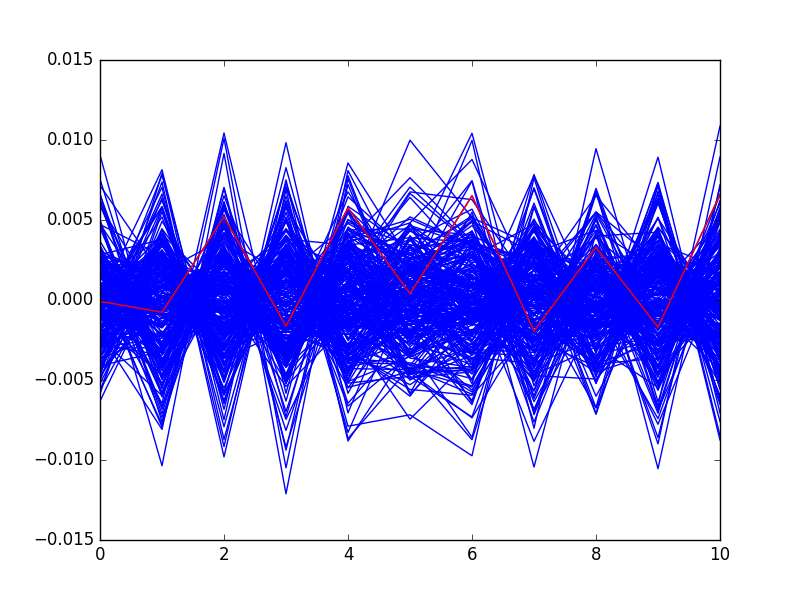
\includegraphics[scale=0.4]{figures/CPA1O_averaged_aZ1.png}
	\caption{Correlation coefficients obtained when targeting $\rmult \times S[\plain[i]\oplus \hat{\key}] \oplus \rout$, on averaged traces, for every value of $\hat{\key}$. Correct hypothesis is plotted in red.}
	\label{fig:CPA1O_averaged_aZ1}
\end{figure}


\subsubsection{Raw Sbox output}
With $50.000$ traces, the attack does not succeed when targeting $S[\plain[i]\oplus \hat{\key}]$.
Figure~\ref{fig:CPA1O_averaged_Z1} illustrates the results using $50.000$ traces.
Figure~\ref{fig:CPA1O_averaged_Z1} illustrates the results using $50.000$ traces.

\begin{figure}[H]
	\centering 
	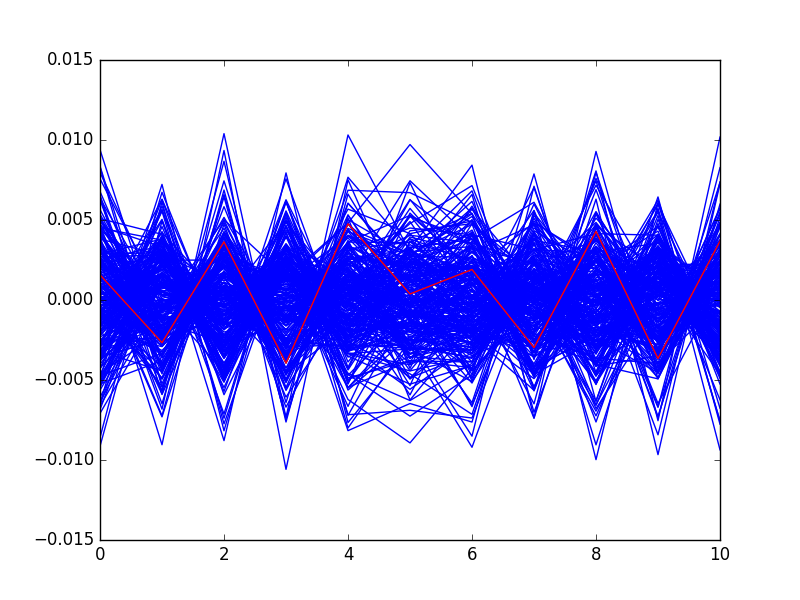
\includegraphics[scale=0.4]{figures/CPA1O_averaged_Z1.png}
	\caption{Correlation coefficients obtained when targeting $\rmult \times S[\plain[i]\oplus \hat{\key}] \oplus \rout$, on averaged traces, for every value of $\hat{\key}$. Correct hypothesis is plotted  in red.}
	\label{fig:CPA1O_averaged_Z1}
\end{figure}

\subsection{Unknown permutation, non-processed traces}

For the sake of completeness, we also perform these experiments on raw unprocessed traces. No success is obtained when targeting $Z_{\hat{\key}}[i]$ or $\rmult \times Z_{\hat{\key}}[i]$ using $50.000$ traces.
Similarly, by targeting $\rmult \times S[\plain[i]\oplus \hat{\key}] \oplus \rout$, the attack does not succeed.


\subsection{Summary}
The results in this section evidence the effectiveness of the implementation of the countermeasures against first-order side-channel attack.
Assuming knowledge of the mask values, the shuffling countermeasure alone increases the number of necessary traces by a factor $\sim 20$.
Furthermore, masking countermeasures seem to completely thwart first order side-channel attacks using $50.000$ traces.


\begin{figure}[h!]
\centering
\begin{tabular}{|c|c|c|c|c|c|c|}
  \hline
   & \multicolumn{3}{c|}{Known permutation}&\multicolumn{3}{c|}{Unknown permutation}\\
  \hline
  Known & $\rmult, \rout$ & $\rmult $ &  None & $\rmult,\rout$ & $\rmult $  &  None \\
  \hline
  \# Traces& $\approx 1.000$ & $ > 50.000$ & $> 50.000$& $\approx 20.000$ & $ > 50.000$ & > $50.000$\\
  \hline
\end{tabular}
\caption{Number of traces needed for a successful first-order attack, in the different settings.}
\end{figure}



\section{Second-order correlation analysis}

In this section, we analyse the effectiveness of the implemented countermeasures against second-order side-channel analysis based on the linear correlation coefficient (CPA). For this study, we will target the Sbox output value and consider a Hamming weight ($HW$) univariate leakage model.

In the remainder of this section, we will use:
\begin{itemize}

\item the centered product combination function $\mathcal{C}(x,y) = (x-\bar{x})(y-\bar{y})$ to preprocess the traces, where $\bar{x}$ (resp. $\bar{y}$) stands for the mean value of $x$ (resp. $y$), computed on all traces in our campaign; 

\item the corresponding function $f_{HW}(z) = \sum_m (HW(z \oplus m) - \overline{HW(z\oplus m)})\\(HW(m)-\overline{HW(m)})$ to compute the predictions, where $\overline{HW(m)}$ (resp $\overline{HW(z \oplus m)}$) stands for the mean value of $HW(m)$ (resp. $HW(z\oplus m)$) computed on all possible values of $m$\footnote{Note that all possible values for $m$ are in $[0,255]$.}.
\end{itemize}

As in our first-order correlation analysis, we will split this study in two parts. The first part will consider priviledged knowledge on the mask values. The second part will not take this knowledge into account.

\subsection{Priviledged knowledge}
We first study the setting where the attacker knows the random masks used to compute the permutation. 
In order to characterize the effectiveness of a CPA against this implementation, we use the random masks to recompute the permutation $Sh(i)$ for each byte index $i$.

For each byte index $i$, we use the characterization phase to isolate a window $w_{z\oplus m}$ of $11$ points of interest corresponding to the manipulation of the Sbox output $\rmult \times S[P[Sh(i)\oplus K[Sh(i)]] \oplus \rout$, and a window $w_m$ of $11$ points of interest corresponding to the manipulation of the mask value $\rout$. For each couple $(i,j)$ of points in $w_{z\oplus m} \times w_m$, we apply the combination function $\mathcal{C}(i,j)$.

\noindent We then perform an attack targeting the value $Z_{\hat{k}}[i]=S[P[Sh(i)] \oplus K[Sh(i)] \oplus \hat{k}]$, where $\hat{k}$ is an hypothesis on a value of one byte.


\subsubsection{Multiplicatively masked Sbox output}
We suppose the knowledge of the multiplicative mask $\rmult$. This knowledge allows for the prediction of the value $\rmult \times Z_{\hat{k}}[i]$ for any hypothesis $\hat{k}$.
The attack succeeds with around $8.000$ traces to $20.000$ traces.
Figure~\ref{fig:CPA2O_trickedaZ1} illustrates the results using $20.000$ traces.

\begin{figure}[H]
	\centering 
	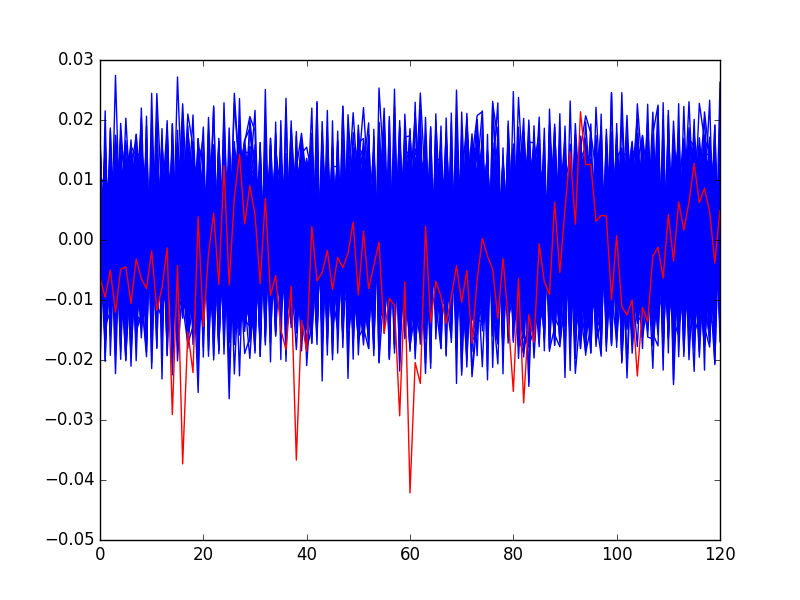
\includegraphics[scale=0.35]{figures/CPA2O_trickedaZ1.png}
	\caption{Correlation coefficients obtained when targeting $\rmult \times S[P[i]\oplus \hat{k}] $, for every value of $\hat{k}$. Correct hypothesis plotted in red. X-axis represents all 121 points combinations.}
	\label{fig:CPA2O_trickedaZ1}
\end{figure}


\subsubsection{Raw Sbox output}
We target the value $Z_{\hat{k}}[i]$ for any hypothesis $k$.
The attack does not succeed using the $100.000$ traces.
Figure~\ref{fig:CPA2O_trickedZ1} illustrates the results using $100.000$ traces.

\begin{figure}[H]
	\centering 
	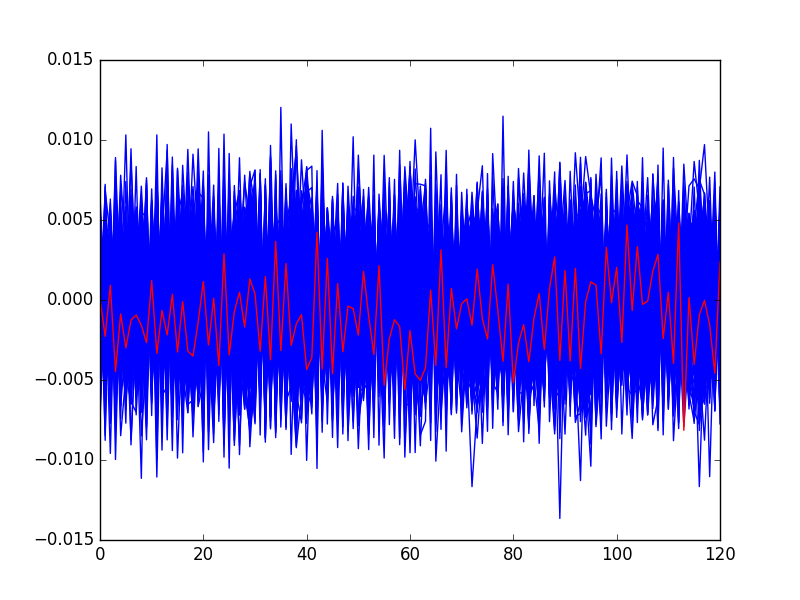
\includegraphics[scale=0.35]{figures/CPA2O_trickedZ1.png}
	\caption{Correlation coefficients obtained when targeting $S[P[i]\oplus \hat{k}] $, for every value of $\hat{k}$. Correct hypothesis plotted in red. X-axis represents all 121 points combinations.}
	\label{fig:CPA2O_trickedZ1}
\end{figure}


\subsection{Unknown permutation, processed traces}
We now study the setting where the attacker does not know the random masks used to compute the permutation.
We preprocess the traces in order to average the leakage over the different byte indices manipulation:
\begin{itemize}
	\item for each index $i$ in $[0,15]$, we define a small window $w_i$ of $\ell$ points around the SNR peak corresponding to the manipulation of $\rmult \times S[P[Sh(i)] \oplus K[Sh(i)]]\oplus \rout$ in the characterization phase. In our experiments, the size of the window was arbitrarily fixed to $\ell=11$.
	\item for each trace in our acquisition campaign, we compute the average window $m$ such that for each time sample $j$, $m[j]=\frac{1}{16}\sum_{i=0}^{15} w_i[j]$. We then consider $m$ as our reduced averaged trace of size $\ell$.
	\item we concatenate to this trace a small window of $\ell$ points around the SNR peak corresponding to the manipulation of $\rout$.
\end{itemize}

\subsubsection{Multiplicatively masked Sbox output}
We suppose the knowledge of the multiplicative mask $\rmult$. This knowledge allows for the prediction of the value $\rmult \times Z_{\hat{k}}[i]$ for any hypothesis $\hat{k}$.
The attack is unsuccessful using $100.000$ traces.

Figure~\ref{fig:CPA2O_averagedaZ1} illustrates the results using $100.000$ traces.
\begin{figure}[H]
	\centering 
	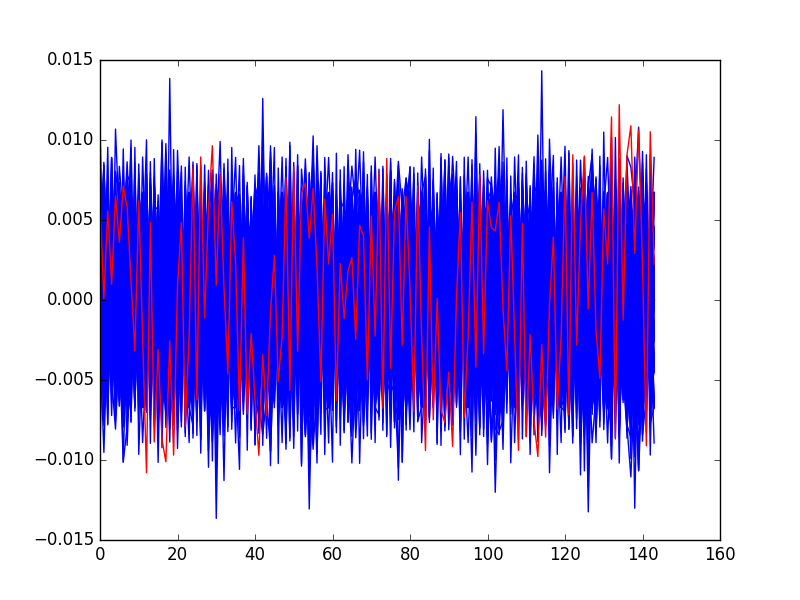
\includegraphics[scale=0.35]{figures/CPA2O_averagedaZ1.png}
	\caption{Correlation coefficients obtained when targeting $\rmult \times S[P[i]\oplus \hat{k}] $, for every value of $\hat{k}$. Correct hypothesis plotted in red. X-axis represents all 121 points combinations.}
	\label{fig:CPA2O_averagedaZ1}
\end{figure}

However, we observe that, for certain combinations of points (around abscissa 135), the correct hypothesis is indeed the most likely. Furthermore, the rank convergence of the key, plotted on Figure~\ref{fig:convergence}, might indicate that the attack could be successful when using more traces.

\begin{figure}[H]
	\centering 
	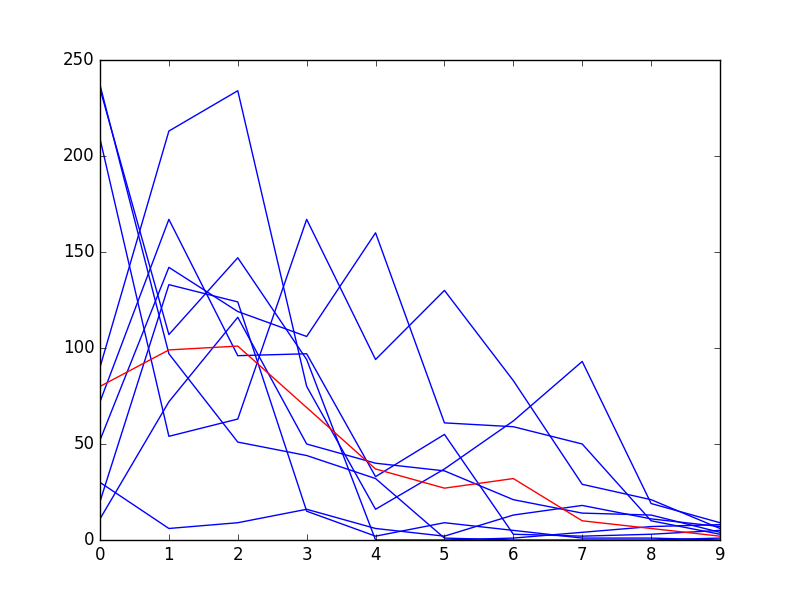
\includegraphics[scale=0.35]{figures/convergence.png}
	\caption{Rank of the ten best-ranked keys, by steps of 10000 measurements, from $10.000$ to $100.000$. Correct key plotted in red.}
	\label{fig:convergence}
\end{figure}

\subsubsection{Raw Sbox output}
We target the value $Z_{\hat{k}}[i]$ for any hypothesis $\hat{k}$.
The attack does not succeed using the $100.000$ traces.
Figure~\ref{fig:CPA2O_averagedZ1} illustrates the results using $100.000$ traces.
\begin{figure}[H]
	\centering 
	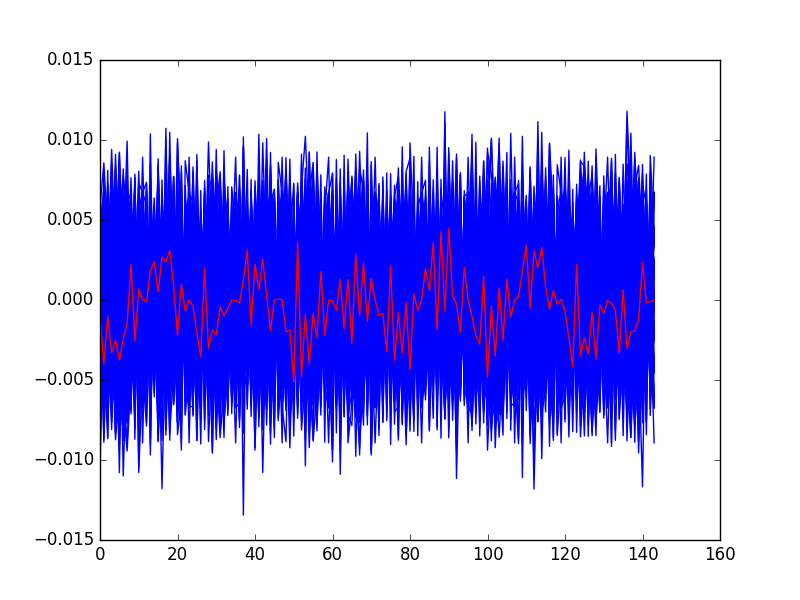
\includegraphics[scale=0.35]{figures/CPA2O_averagedZ1.png}
	\caption{Correlation coefficients obtained when targeting $S[P[i]\oplus \hat{k}] $, for every value of $\hat{k}$. Correct hypothesis plotted in red. X-axis represents all 121 points combinations.}
	\label{fig:CPA2O_averagedZ1}
\end{figure}


\subsection{Unknown permutation, non-processed traces}
For the sake of completeness, we also perform these experiments on raw unprocessed traces. No success is obtained when targeting $Z_{\hat{k}}[i]$ or $\rmult \times Z_{\hat{k}}[i]$.

No attack is successful using $100.000$ traces.

\subsection{Summary}
This section evidences the effectiveness of the implemented countermeasures. 
The shuffling countermeasures increases the number of needed measurements by a factor of at least $\frac{100.000}{8.000} = 12,5$. It is however likely that this countermeasure does not suffice when increasing slightly the number of measurements.
The effectiveness of the affine countermeasure is evidenced by the fact that a 2OCPA is achievable targeting the value $\rmult \times S[P[i] \oplus \hat{k}]$
but no attack is found targeting the value $S[P[i] \oplus \hat{k}]$ using $100.000$ traces.

\begin{figure}[h!]
\centering
\begin{tabular}{|c|c|c|c|c|}
  \hline
   & \multicolumn{2}{c|}{Known permutation}&\multicolumn{2}{c|}{Unknown permutation}\\
  \hline
  Known & $\rmult $ &  None  & $\rmult $  &  None \\
  \hline
  \# Traces& $\approx 8.000$ & $ > 100.000$ & $ > 100.000$ & $> 100.000$\\
  \hline
\end{tabular}
\caption{Number of traces needed for a successful second-order attack, in the different settings.}
\end{figure}




\section{Third-order correlation analysis}

In this section, we analyse the resistance of the implementation against third order side-channel analysis based on the linear correlation coefficient (CPA). For this study, we will target the Sbox output value and consider a Hamming weight ($HW$) univariate leakage model.

In the remainder of this section, we will use:
\begin{itemize}

\item the centered product combination function $\mathcal{C}(x,y,z) = (x-\overline{x})(y-\overline{y})(z-\bar{z})$ to preprocess the traces, where $\overline{x}$ (resp. $\overline{y}$, $\bar{z}$) stands for the mean value of $x$ (resp. $y$, $z$), computed on all traces in our campaign; 

\item the corresponding function $f_{HW}(z) = \sum_{m,m'} (HW(m'\times z \oplus m) -\\ \overline{HW(m'\times z\oplus m)})(HW(m)-\overline{HW(m)})(HW(m')-\overline{HW(m')})$ to compute the predictions, where $\overline{HW(m)}$ (resp $\overline{HW(m'\times z \oplus m)}$, $\overline{HW(m')}$) stands for the mean value of $HW(m)$ (resp. $HW(m' \times z\oplus m)$, $HW(m')$) computed on all possible values of $m,m'$\footnote{Note that all possible values for $m$ are in $[0,255]$, while all possible values for $m'$ are in $[1,255]$.}.
\end{itemize}

As in our first-order and second-order correlation analyses, we will split this study in two parts. The first part will consider priviledged knowledge on the mask values. The second part will not consider this knowledge.

\subsection{Priviledged knowledge}
We first study the setting where the attacker knows the random masks used to compute the permutation. 

In order to characterize the effectiveness of a CPA against this implemenation, we use the random masks to recompute the permutation $Sh(i)$ for each byte index $i$.

\subsubsection{Raw Sbox output}
We target the value $Z_{\hat{k}}[i]$ for any hypothesis $k$.
The attack does not succeed using the $100.000$ traces.
%/media/nas/projects/ASCAD_CW/ASCAD_ChipWhisperer/ARM/traces/attack_results_3O_without_flaw_fixed_100k.h5
Figure~\ref{fig:CPA3O_trickedZ1} illustrates the results using $100000$ traces.
\begin{figure}[H]
	\centering 
	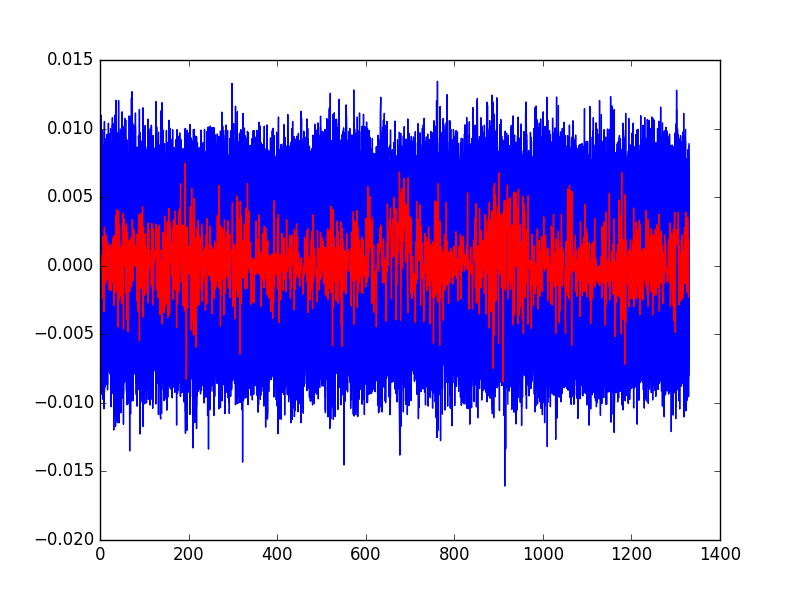
\includegraphics[scale=0.35]{figures/CPA3O_trickedZ1.png}
	\caption{Correlation coefficients obtained when targeting $S[P[i]\oplus \hat{k}] $, for every value of $\hat{k}$. Correct hypothesis plotted in red. X-axis represents all 1331 points combinations.}
	\label{fig:CPA3O_trickedZ1}
\end{figure}

\subsection{Unknown permutation, processed traces}
We now study the setting where the attacker does not know the random masks used to compute the permutation.

We preprocess the traces in order to average the leakage over the different byte indices manipulation:
\begin{itemize}
	\item for each index $i$ in $[0,15]$, we define a small window $w_i$ of $\ell$ points around the SNR peak corresponding to the manipulation of $\rmult \times S[P[Sh(i)] \oplus K[Sh(i)]]\oplus \rout$ in the characterization phase. In our experiments, the size of the window was arbitrarily fixed to $\ell=11$.
	\item for each trace in our acquisition campaign, we compute the average window $m$ such that for each time sample $j$, $m[j]=\frac{1}{16}\sum_{i=0}^{15} w_i[j]$. We then consider $m$ as our reduced averaged trace of size $\ell$.
	\item we concatenate to this trace a small window of $\ell$ points around the SNR peak corresponding to the manipulation of $\rout$.
\end{itemize}


\subsubsection{Raw Sbox output}
We target the value $Z_{\hat{k}}[i]$ for any hypothesis $k$.
The attack does not succeed using the $100.000$ traces. The correct key rank does not seem to indicate that this number of traces is close to allow a success attack.
Figure~\ref{fig:CPA3O_averagedZ1} illustrates the results using $100.000$ traces.

\begin{figure}[H]
	\centering 
	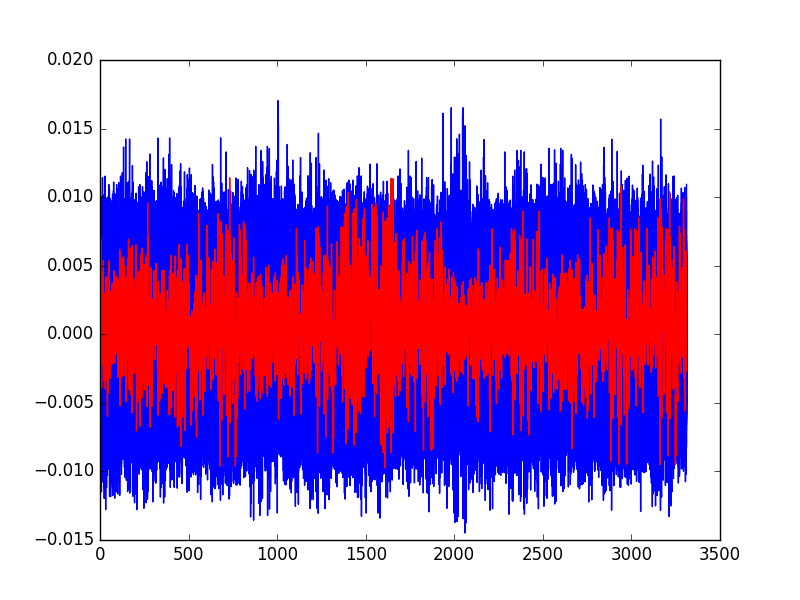
\includegraphics[scale=0.35]{figures/CPA3O_averagedZ1.png}
	\caption{Correlation coefficients obtained when targeting $S[P[i]\oplus \hat{k}] $, for every value of $\hat{k}$. Correct hypothesis plotted in red. X-axis represents all 1331 points combinations.}
	\label{fig:CPA3O_averagedZ1}
\end{figure}


\subsection{Unknown permutation, non-processed traces}
For the sake of completeness, we also perform these experiments on raw unprocessed traces. No success is obtained when targeting $Z_{\hat{k}}[i]$.
No attack is successful using $100.000$ traces.
Figure~\ref{fig:CPA3O_rawZ1} illustrates the results using $100.000$ traces.
\begin{figure}[H]
	\centering 
	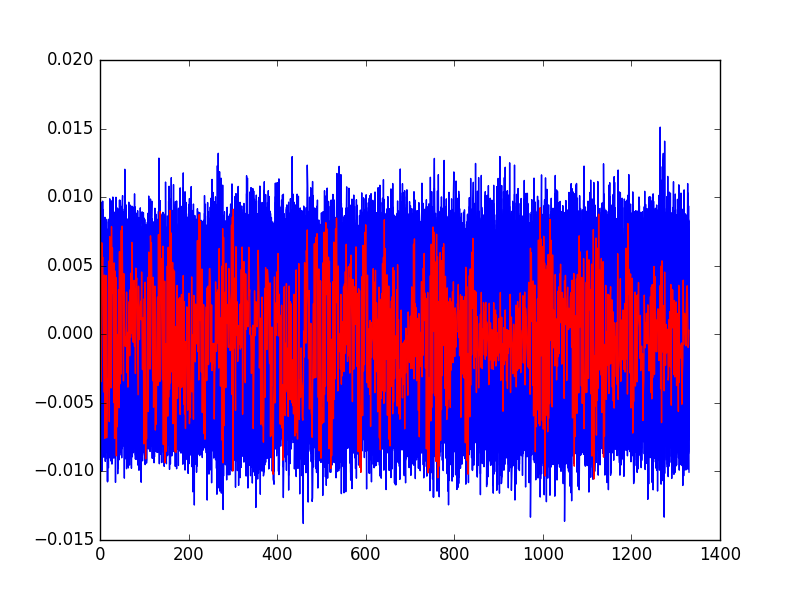
\includegraphics[scale=0.35]{figures/CPA3O_rawZ1.png}
	\caption{Correlation coefficients obtained when targeting $S[P[i]\oplus \hat{k}] $, for every value of $\hat{k}$. Correct hypothesis plotted in red. X-axis represents all 1331 points combinations.}
	\label{fig:CPA3O_rawZ1}
\end{figure}

\subsection{Summary}
No third order attack has been achieved using $100.000$ traces.


%\newpage
\bibliographystyle{plain}
\bibliography{ANSSI}

\end{document}
